%==============================================================================
% tento soubor pouzijte jako zaklad
% this file should be used as a base for the thesis
% Autoři / Authors: 2008 Michal Bidlo, 2019 Jaroslav Dytrych
% Kontakt pro dotazy a připomínky: sablona@fit.vutbr.cz
% Contact for questions and comments: sablona@fit.vutbr.cz
%==============================================================================
% kodovani: UTF-8 (zmena prikazem iconv, recode nebo cstocs)
% encoding: UTF-8 (you can change it by command iconv, recode or cstocs)
%------------------------------------------------------------------------------
% zpracování / processing: make, make pdf, make clean
%==============================================================================
% Soubory, které je nutné upravit nebo smazat: / Files which have to be edited or deleted:
%   projekt-20-literatura-bibliography.bib - literatura / bibliography
%   projekt-01-kapitoly-chapters.tex - obsah práce / the thesis content
%   projekt-01-kapitoly-chapters-en.tex - obsah práce v angličtině / the thesis content in English
%   projekt-30-prilohy-appendices.tex - přílohy / appendices
%   projekt-30-prilohy-appendices-en.tex - přílohy v angličtině / appendices in English
%==============================================================================
\documentclass[slovak, zadani]{fitthesis} % bez zadání - pro začátek práce, aby nebyl problém s překladem
%\documentclass[english]{fitthesis} % without assignment - for the work start to avoid compilation problem
%\documentclass[zadani]{fitthesis} % odevzdani do wisu a/nebo tisk s barevnými odkazy - odkazy jsou barevné
%\documentclass[english,zadani]{fitthesis} % for submission to the IS FIT and/or print with color links - links are color
%\documentclass[zadani,print]{fitthesis} % pro černobílý tisk - odkazy jsou černé
%\documentclass[english,zadani,print]{fitthesis} % for the black and white print - links are black
%\documentclass[zadani,cprint]{fitthesis} % pro barevný tisk - odkazy jsou černé, znak VUT barevný
%\documentclass[english,zadani,cprint]{fitthesis} % for the print - links are black, logo is color
% * Je-li práce psaná v anglickém jazyce, je zapotřebí u třídy použít 
%   parametr english následovně:
%   If thesis is written in English, it is necessary to use 
%   parameter english as follows:
%      \documentclass[english]{fitthesis}
% * Je-li práce psaná ve slovenském jazyce, je zapotřebí u třídy použít 
%   parametr slovak následovně:
%   If the work is written in the Slovak language, it is necessary 
%   to use parameter slovak as follows:
%      \documentclass[slovak]{fitthesis}
% * Je-li práce psaná v anglickém jazyce se slovenským abstraktem apod., 
%   je zapotřebí u třídy použít parametry english a enslovak následovně:
%   If the work is written in English with the Slovak abstract, etc., 
%   it is necessary to use parameters english and enslovak as follows:
%      \documentclass[english,enslovak]{fitthesis}

% Základní balíčky jsou dole v souboru šablony fitthesis.cls
% Basic packages are at the bottom of template file fitthesis.cls
% zde můžeme vložit vlastní balíčky / you can place own packages here

% Kompilace po částech (rychlejší, ale v náhledu nemusí být vše aktuální)
% Compilation piecewise (faster, but not all parts in preview will be up-to-date)
% \usepackage{subfiles}

% Nastavení cesty k obrázkům
% Setting of a path to the pictures
\graphicspath{{obrazky-figures/}{./obrazky-figures/}}
\graphicspath{{obrazky-figures/}{../obrazky-figures/}}

%---rm---------------
\renewcommand{\rmdefault}{lmr}%zavede Latin Modern Roman jako rm / set Latin Modern Roman as rm
%---sf---------------
\renewcommand{\sfdefault}{qhv}%zavede TeX Gyre Heros jako sf
%---tt------------
\renewcommand{\ttdefault}{lmtt}% zavede Latin Modern tt jako tt

% vypne funkci šablony, která automaticky nahrazuje uvozovky,
% aby nebyly prováděny nevhodné náhrady v popisech API apod.
% disables function of the template which replaces quotation marks
% to avoid unnecessary replacements in the API descriptions etc.
\csdoublequotesoff



\usepackage{url}
\usepackage{nomencl}
\makenomenclature

% =======================================================================
% balíček "hyperref" vytváří klikací odkazy v pdf, pokud tedy použijeme pdflatex
% problém je, že balíček hyperref musí být uveden jako poslední, takže nemůže
% být v šabloně
% "hyperref" package create clickable links in pdf if you are using pdflatex.
% Problem is that this package have to be introduced as the last one so it 
% can not be placed in the template file.
\ifWis
\ifx\pdfoutput\undefined % nejedeme pod pdflatexem / we are not using pdflatex
\else
  \usepackage{color}
  \usepackage[unicode,colorlinks,hyperindex,plainpages=false,pdftex]{hyperref}
  \definecolor{hrcolor-ref}{RGB}{223,52,30}
  \definecolor{hrcolor-cite}{HTML}{2F8F00}
  \definecolor{hrcolor-urls}{HTML}{092EAB}
  \hypersetup{
	linkcolor=hrcolor-ref,
	citecolor=hrcolor-cite,
	filecolor=magenta,
	urlcolor=hrcolor-urls
  }
  \def\pdfBorderAttrs{/Border [0 0 0] }  % bez okrajů kolem odkazů / without margins around links
  \pdfcompresslevel=9
\fi
\else % pro tisk budou odkazy, na které se dá klikat, černé / for the print clickable links will be black
\ifx\pdfoutput\undefined % nejedeme pod pdflatexem / we are not using pdflatex
\else
  \usepackage{color}
  \usepackage[unicode,colorlinks,hyperindex,plainpages=false,pdftex,urlcolor=black,linkcolor=black,citecolor=black]{hyperref}
  \definecolor{links}{rgb}{0,0,0}
  \definecolor{anchors}{rgb}{0,0,0}
  \def\AnchorColor{anchors}
  \def\LinkColor{links}
  \def\pdfBorderAttrs{/Border [0 0 0] } % bez okrajů kolem odkazů / without margins around links
  \pdfcompresslevel=9
\fi
\fi
% Řešení problému, kdy klikací odkazy na obrázky vedou za obrázek
% This solves the problems with links which leads after the picture
\usepackage[all]{hypcap}

% Informace o práci/projektu / Information about the thesis
%---------------------------------------------------------------------------
\projectinfo{
  %Prace / Thesis
  project={BP},            %typ práce BP/SP/DP/DR  / thesis type (SP = term project)
  year={2022},             % rok odevzdání / year of submission
  date=\today,             % datum odevzdání / submission date
  %Nazev prace / thesis title
  title.cs={Grafické rozhranie priehľadového displeja},  % název práce v češtině či slovenštině (dle zadání) / thesis title in czech language (according to assignment)
  title.en={Graphical Interface for Head-Up Display}, % název práce v angličtině / thesis title in english
  %title.length={14.5cm}, % nastavení délky bloku s titulkem pro úpravu zalomení řádku (lze definovat zde nebo níže) / setting the length of a block with a thesis title for adjusting a line break (can be defined here or below)
  %sectitle.length={14.5cm}, % nastavení délky bloku s druhým titulkem pro úpravu zalomení řádku (lze definovat zde nebo níže) / setting the length of a block with a second thesis title for adjusting a line break (can be defined here or below)
  %dectitle.length={14.5cm}, % nastavení délky bloku s titulkem nad prohlášením pro úpravu zalomení řádku (lze definovat zde nebo níže) / setting the length of a block with a thesis title above declaration for adjusting a line break (can be defined here or below)
  %Autor / Author
  author.name={Slavomír},   % jméno autora / author name
  author.surname={Svorada},   % příjmení autora / author surname 
  %author.title.p={Bc.}, % titul před jménem (nepovinné) / title before the name (optional)
  %author.title.a={Ph.D.}, % titul za jménem (nepovinné) / title after the name (optional)
  %Ustav / Department
  department={UPGM}, % doplňte příslušnou zkratku dle ústavu na zadání: UPSY/UIFS/UITS/UPGM / fill in appropriate abbreviation of the department according to assignment: UPSY/UIFS/UITS/UPGM
  % Školitel / supervisor
  supervisor.name={Peter},   % jméno školitele / supervisor name 
  supervisor.surname={Chudý},   % příjmení školitele / supervisor surname
  supervisor.title.p={doc. Ing.},   %titul před jménem (nepovinné) / title before the name (optional)
  supervisor.title.a={Ph.D. MBA},    %titul za jménem (nepovinné) / title after the name (optional)
  % Klíčová slova / keywords
  keywords.cs={letové veličiny, priehľadový displej, letecký simulátor, virtuálna realita, letové dáta, letectvo}, % klíčová slova v českém či slovenském jazyce / keywords in czech or slovak language
  keywords.en={flight quantities, head-up display, flight simulator, virtual reality, flight data, aviation}, % klíčová slova v anglickém jazyce / keywords in english
  %keywords.en={Here, individual keywords separated by commas will be written in English.},
  % Abstrakt / Abstract
  abstract.cs={Táto práca sa zaoberá trendami v oblasti vizualizácie letových dát. Cieľom práce je navrhnúť vlastnú vizualizáciu letových dát pre priehľadový displej a následne návrh implementovať v prostredí leteckého simulátora, ktorý obsahuje technológie podporujúce virtuálnu realitu. Špecifickým zámerom bolo vytvorenie priehľadového displeja pre elektrický letún s kolmým štartom a pristátim (eVTOL).}, % abstrakt v českém či slovenském jazyce / abstract in czech or slovak language
  abstract.en={This work deals with trends in the field of flight data visualization. The aim of the work is to design own visualization of flight data for a head-up display and then implement the proposal in a flight simulator environment, which contains technologies that support virtual reality. The specific intention was creating a head-up display for the electric plane with vertical take-off and landing (eVTOL).}, % abstrakt v anglickém jazyce / abstract in english
  %abstract.en={An abstract of the work in English will be written in this paragraph.},
  % Prohlášení (u anglicky psané práce anglicky, u slovensky psané práce slovensky) / Declaration (for thesis in english should be in english)
  declaration={Prehlasujem, že som túto bakalársku prácu vypracoval samostatne pod vedením pána doc. Ing. Petera Chudého, Ph.D., MBA
Uviedol som všetky literárne pramene a publikácie, z~ktorých som čerpal.},
  %declaration={I hereby declare that this Bachelor's thesis was prepared as an original work by the author under the supervision of Mr. X
% The supplementary information was provided by Mr. Y
% I have listed all the literary sources, publications and other sources, which were used during the preparation of this thesis.},
  % Poděkování (nepovinné, nejlépe v jazyce práce) / Acknowledgement (optional, ideally in the language of the thesis)
  acknowledgment={Chcel by som sa poďakovať doc. Ing. Petrovi Chudému, Ph.D., MBA za ochotu, čas a cenné rady, ktoré mi poskytol počas tvorby tejto bakalárskej práce.},
  %acknowledgment={Here it is possible to express thanks to the supervisor and to the people which provided professional help
%(external submitter, consultant, etc.).},
  % Rozšířený abstrakt (cca 3 normostrany) - lze definovat zde nebo níže / Extended abstract (approximately 3 standard pages) - can be defined here or below
  %extendedabstract={Do tohoto odstavce bude zapsán rozšířený výtah (abstrakt) práce v českém (slovenském) jazyce.},
  %extabstract.odd={true}, % Začít rozšířený abstrakt na liché stránce? / Should extended abstract start on the odd page?
  %faculty={FIT}, % FIT/FEKT/FSI/FA/FCH/FP/FAST/FAVU/USI/DEF
  faculty.cs={Fakulta informačních technologií}, % Fakulta v češtině - pro využití této položky výše zvolte fakultu DEF / Faculty in Czech - for use of this entry select DEF above
  faculty.en={Faculty of Information Technology}, % Fakulta v angličtině - pro využití této položky výše zvolte fakultu DEF / Faculty in English - for use of this entry select DEF above
  department.cs={Ústav matematiky}, % Ústav v češtině - pro využití této položky výše zvolte ústav DEF nebo jej zakomentujte / Department in Czech - for use of this entry select DEF above or comment it out
  department.en={Institute of Mathematics} % Ústav v angličtině - pro využití této položky výše zvolte ústav DEF nebo jej zakomentujte / Department in English - for use of this entry select DEF above or comment it out
}

% Rozšířený abstrakt (cca 3 normostrany) - lze definovat zde nebo výše / Extended abstract (approximately 3 standard pages) - can be defined here or above
%\extendedabstract{Do tohoto odstavce bude zapsán výtah (abstrakt) práce v českém (slovenském) jazyce.}
% Začít rozšířený abstrakt na liché stránce? / Should extended abstract start on the odd page?
%\extabstractodd{true}

% nastavení délky bloku s titulkem pro úpravu zalomení řádku - lze definovat zde nebo výše / setting the length of a block with a thesis title for adjusting a line break - can be defined here or above
%\titlelength{14.5cm}
% nastavení délky bloku s druhým titulkem pro úpravu zalomení řádku - lze definovat zde nebo výše / setting the length of a block with a second thesis title for adjusting a line break - can be defined here or above
%\sectitlelength{14.5cm}
% nastavení délky bloku s titulkem nad prohlášením pro úpravu zalomení řádku - lze definovat zde nebo výše / setting the length of a block with a thesis title above declaration for adjusting a line break - can be defined here or above
%\dectitlelength{14.5cm}

% řeší první/poslední řádek odstavce na předchozí/následující stránce
% solves first/last row of the paragraph on the previous/next page
\clubpenalty=10000
\widowpenalty=10000

% checklist
\newlist{checklist}{itemize}{1}
\setlist[checklist]{label=$\square$}

% Nechcete-li, aby se u oboustranného tisku roztahovaly mezery pro zaplnění stránky, odkomentujte následující řádek / If you do not want enlarged spacing for filling of the pages in case of duplex printing, uncomment the following line
% \raggedbottom

\begin{document}
  % Vysazeni titulnich stran / Typesetting of the title pages
  % ----------------------------------------------
  \maketitle
  % Obsah
  % ----------------------------------------------
  \setlength{\parskip}{0pt}

  {\hypersetup{hidelinks}\tableofcontents}
  
  % Seznam obrazku a tabulek (pokud prace obsahuje velke mnozstvi obrazku, tak se to hodi)
  % List of figures and list of tables (if the thesis contains a lot of pictures, it is good)
  \ifczech
    \renewcommand\listfigurename{Seznam obrázků}
  \fi
  \ifslovak
    \renewcommand\listfigurename{Zoznam obrázkov}
  \fi
     {\hypersetup{hidelinks}\listoffigures}
\nomenclature{ACM}{Air Combat Manoeuvre - (Vzdušný bojový manéver)}
\nomenclature{AGL}{Above Ground Level - (Nad úrovňou zeme)}
\nomenclature{ALT}{Altitude - (Nadmorská výška)}
\nomenclature{ASI}{Airspeed Indicator - (Rýchlomer)}
\nomenclature{CAS}{Calibrated Air Speed - (Kalibrovaná vzdušná rýchlosť)}
\nomenclature{EVS}{Enhanced Vision System - (Systém vylepšeného videnia)}
\nomenclature{eVTOL}{electric Vertical Takeoff and Landing - (Vertikálny odlet a pristátie)}
\nomenclature{GS}{Ground Speed - (Rýchlosť voči zemi)}
\nomenclature{HMD}{Helmet Mounted Display - (Prilbový displej)}
\nomenclature{HUD}{Head Up Display - (Priehľadový displej)}
\nomenclature{IAS}{Indicated Airspeed - (Indikovaná vzdušná rýchlosť)}
\nomenclature{ILS}{Instrument Landing System - (Prístrojový pristávací systém)}
\nomenclature{KIAS}{Knots Indicated Airspeed - (Uzly indikovanej rýchlosti)}
\nomenclature{QNH}{Kód pre tlak vzduchu prepočítaný na hladinu mora}
\nomenclature{SDO}{Spatial Disorientation - (Priestorová dezorientácia)}
\nomenclature{SVS}{Synthetic Vision System - (Systém syntetického videnia)}
\nomenclature{STD}{Skratka pre nastavenie tlaku vzduchu. Reprezentuje hodnotu 1013 hPa}
\nomenclature{TAS}{True Airspeed - (Pravá vzdušná rýchlosť)}
\nomenclature{USAF}{United States Air Force - (Letectvo Spojených štátov amerických)}
\nomenclature{VR}{Virtual Reality - (Virtuálna realita)}
\nomenclature{VSI}{Vertical Speed Indicator - (Indikátor vertikálnej rýchlosti)}
\nomenclature{FSF}{Flight Safety Foundation - (Organizácia pre bezpečnosť letectva)}
\nomenclature{FPM}{Flight Path Marker - (Značka dráhy letu)}

\renewcommand{\nomname}{Zoznam skratiek}
\printnomenclature
  \ifczech
    \renewcommand\listtablename{Seznam tabulek}
  \fi
  \ifslovak
    \renewcommand\listtablename{Zoznam tabuliek}
  \fi
  % {\hypersetup{hidelinks}\listoftables}

  \ifODSAZ
    \setlength{\parskip}{0.5\bigskipamount}
  \else
    \setlength{\parskip}{0pt}
  \fi

  % vynechani stranky v oboustrannem rezimu
  % Skip the page in the two-sided mode
  \iftwoside
    \cleardoublepage
  \fi
  % Text prace / Thesis text
  % ----------------------------------------------
  \ifenglish
    \input{projekt-01-kapitoly-chapters-en}
  \else
    % Autor: Slavomír Svorada 
% Popis: Bakalárska práca
% Téma: Grafické rozhranie priehľadového displeja

%----------------------------UVOD-----------------------------------
\chapter{Úvod}
V~súčasnosti nie je priehľadový displej žiadnou novinkou. Jedná sa o~displej, na ktorom sú zobrazované dôležité údaje týkajúce sa letúna. Vďaka priehľadovému displeju nemusí pilot skladať oči z~vonkajšieho okolia a všetky dôležité informácie má k~dispozícii vo svojom zornom poli. S~priehľadovými displejmi sa okrem letúnov môžeme stretnúť aj na palubných doskách automobilov.

Táto práca sa zaoberá trendmi v~oblasti vizualizácie letových dát. Cieľom práce je navrhnúť vlastnú vizualizáciu letových dát pre priehľadový displej a následne návrh implementovať v~prostredí leteckého simulátora, ktorý obsahuje technológie podporujúce virtuálnu realitu. Hlavné zameranie je vytvoriť priehľadový displej pre elektrický letún s~kolmým štartom a~pristátim (eVTOL). Dôvod výberu tohto letúna bol ten, že uvedený typ letúnov patrí medzi najmodernejšie \cite{eVTOL}. Tým, že priehľadový displej je implementovaný v~leteckom simulátore, ktorý podporuje virtuálnu realitu, tak riešenie je veľmi efektívne pri viacerých manévroch.

Druhá kapitola bakalárskej práce pojednáva o~historickom vývoji návrhu vizualizácie letových veličín v~pilotnej kabíne. V~tejto kapitole je zhrnutý vývoj priehľadového displeja (HUD) od skorého začiatku. Taktiež sú v~tejto kapitole spomenuté základné letové prístroje letúnov. Je tu spomenutý balíček šiestich prístrojov, ktoré sú súčasťou každého letúna. V~následujúcej tretej kapitole sú popísané súčasne trendy vizualizácie letových dát. V~kapitole sú popísané tri typy displejov a to Head Down Display (HDD), Head Up Display (HUD) a~Helmet Mounted Display (HMD). Pri HDD sú vysvetlené dva typy displejov a to primárny letový displej a multifunkčný displej. V~kapitole je následne spomenutý základný popis priehľadového displeja. Ďalej sú popísane jeho jednotlivé komponenty. Následne sú spomenuté jednotlivé generácie HUD, stav súčasných HUD v~letectve, symbolika HUD a~nakoniec je spomenutý popis prilbového displeja (HMD) s~adresovanými výhodami a nevýhodami. Vo~štvrtej kapitole sa nachádza návrh vizualizácie letových dát pre priehľadový displej. Na začiatku kapitoli je spomenutá štruktúra systému. V~kapitole je prezentovaný postupný vývoj jednotlivých návrhov HUD. Sú tu taktiež podrobnejšie popísané jednotlivé časti posledného navrhovaného displeja. Popis implementácie sa nachádza v~piatej kapitole. Šiesta kapitola obsahuje testovanie v~prostredí leteckého simulátora a výsledky práce. V~poslednej siedmej kapitole je spomenutý záver práce a taktiež sú tu spomenuté možnosti budúceho vývoja.\newpage

%----------------------------HISTORIA-----------------------------------
\chapter{Historický vývoj návrhu vizualizácie letových veličín v~pilotnej kabíne} 
\label{struktura}
Od začiatku vývoja letectva je známe, že poskytovanie informácií pilotovi o~letúne môže byť užitočné a viesť k~bezpečnejšiemu letu. Medzi dôležité orientačné body a udalosti na ceste k~vynálezu letúna patrí pochopenie dynamickej reakcie krídel, konštrukcia spoľahlivých motorov, ktoré produkujú dostatočný výkon pre letún. Bratia Wrightovci mali na svojom letúne len veľmi málo prístrojov. Keď na začiatku 20. storočia ukázali, že základné technické problémy boli prekonané, vojenské a civilné letectvo sa rýchlo rozvinulo \cite{historia}.

% Historia prehlad kniha
\section{Historický rozhľad priehľadového displeja}
Prvé priehľadové displeje (HUD) boli vyvinuté vo viacerých krajinách koncom 50. rokov 20. storočia. Boli založené na technológií reflexných zameriavačov. V~týchto mieridlách je zameriavaci symbol generovaný zo svetelného zdroja a je premietaný na polopriepustné zrkadlo, ktoré je namontované medzi pilotom a čelným sklom. Projektor sa zvyčajne nachádza v~hornej časti prístrojového panela. Z~pohľadu pilota sa zdá, akoby bol system mierenia zobrazovaný vo vonkajšom svete \cite{HUDkniha}. 

Reflexné zameriavače boli prvykrát použité v~stíhacích letúnoch v~druhej svetovej vojne. Ku koncu 50. rokov 20. storočia sa pokročilo ku zobrazovaniu obrázkov generovaných na~katódových trubiciach (CRT), ktoré boli riadené palubným počítačom. Tieto zameriavače majú niekoľko výhod oproti ich predchádzajúcim nepohyblivým mieridlám. V~prvom rade je možné posunúť zameriavaci symbol tak, aby sa kompenzoval dosah, pokles strely či faktory zrýchlenia. Zo začlenením palubných počítačov, sa rovnice pohybu symbolov stali dosť zložitými. Druhá výhoda je, že obraz zameriavacieho symbolu môže byť zameraný na~vytvorenie obrazu, ktorý vyzerá, akoby ležal v~rovnakej rovine ako cieľ. Uvedená výhoda minimalizuje potrebu pilota sústrediť sa na dve vzdialenosti, čo eliminuje prípadné chyby. Treťou výhodou je možnosť upravenia jasu zameravacieho symbolu, čo môže byť vykonané manuálne alebo automaticky \cite{HUDkniha}.

Ďalším krokom vo vývoji HUD bolo pridanie letových informácií. Hlavným cieľom vývoja HUD bolo umiestnenie letových informácií do priestoru zorného pola pilota. Pôvodne sa o~tom uvažovalo už počas obdobia bojov, kedy by táto pomôcka dokázala zlepšiť schopnosti pilota \cite{HUDkniha}.

Začiatkom šesťdesiatych rokov 20. storočia boli priehľadové displeje vnímané ako pomôcka pre pilotov počas pristávania. Ďalším dôvodom vývoja HUD bola integrácia veľkého počtu samostatných prístrojov nachádzajúcich sa na palubnej doske letúna do jedného displeja \cite{HUDkniha}.

\subsection{Prevádzkové problémy}
V~súčastosti sa nachádzajú priehľadové displeje na väčšine stíhacích alebo útočných letúnoch. Pri prvých použitiach HUD na týchto letúnoch slúžili tieto displeje hlavne ako zameriavače. Časom piloti zistili, že HUD je mimoriadne užitočný a nápomocný aj pri bežnom lete. Piloti USAF lietajúci na letúnoch A-7D a F-15 uviedli, že používajú HUD ako dôležitú časť pre získanie rozličných údajov \cite{HUDknihaproblemy}.

Začiatkom osemdesiatych rokov sa uskutočnil ďalší program na vývoj nových, štandardizovaných kritétií HUD. Ako súčasť tohto úsilia bola pripravená konštručná príručka, ktorá mala pomôcť konštruktérom vytvoriť HUD a zabezpečiť, aby ďalšia generácia displejov bola vhodná pre misijné úlohy \cite{HUDknihaproblemy}.

História nehôd moderných letúnov naznačuje, že priestorová dezorientácia (SDO) je~hlavným problémom vo vojenských letúnoch. Pomerne často je obviňovaný HUD z~toho, že spôsobil dezorientáciu pilota \cite{HUDknihaproblemy}.

\subsection{Vývoj priehľadového displeja}
Veľká časť prvotného vývoja priehľadových displejov sa uskutočnila koncom 50. a začiatkom šesťdesiatych rokov 20. storočia v~britskom Royal Aircraft Establishment (RAE). Tento vývoj prevažne viedol Naish \cite{HUDkniha}. Neskôr ku koncu šesťdesiatych rokov pokračoval vo vývoji priehľadového displeja pre letún Douglas \cite{HUDkniha}.

Briti používali HUD, ktorý obsahoval jednu horizontálnu čiaru a referenčný symbol letúna. V~displejoch tohto typu je rýchlosť a výška letúna zobrazená digitálne. Britská škola navrhla, že HUD nemusí byť v~súlade so skutočným svetom. Ich výsledky boli založené na~rozsiahlom testovaní na simulátoroch. Kritériom úspechu pre väčšinu experimentov bolo sledovanie schopnosti pilota. V~jednom experimente však Naish zámerne naviedol niektorých pilotov na pristátie na jednu stranu pristávacej dráhy. Zistil, že piloti mali tendenciu ignorovať HUD a lietať podľa podnetov z~reálneho sveta hneď, ako boli dostupné. Ďalším vyvodeným záverom bolo, že mierka 1:1 nemusí nevyhnutne priniesť najlepší výkon pilota. Toto pozorovanie malo vplyv na HUD stíhacich letúnoch typu Harrier, kde používali mierku 5:1 \cite{HUDkniha}.

V~polovici šesťdesiatych rokov 20. storočia pokračovali v~USA ďalšie práce, najmä Sperry s~podporov amerického námorníctva. Táto práca, vedená Goldom zdôraznila dva aspekty HUD a to použitie displeja pri vizuálnych priblíženiach pri pristávaní a nevyhnutné optické kvality displeja. Gold \cite{4502188} dospel k~záveru, že pri vizuálnom priblížení bola jediná riadená nápoveda, ktorú pilot používal až do pristátia letúna lepšia, ako kombinácia značky dráhy letu mierky cieľového zostupu. K~rovnakému záveru sa dospelo aj v~následujúcich štúdiach~\cite{39}.

\subsubsection{Vojenské aplikácie}
Začiatkom sedemdesiatych rokov sa koncepcia HUD rozvinula do takej miery, že by mohla byť súčasťou systémov dodávky zbraní pre vojenské stíhacie letúny. Medzi prvé dve významné americké letúny, ktoré používali priehľadové displeje, boli A-7D/E a AV-8A. Obe boli jednomiestne bojové letúny. Hlavnou motiváciou použitia HUD bola modernizácia bombových zameriavačov používaných v~predchádzajúcich útočných letúnoch. Oba modely stíhacich letúnov sú zobrazené na obrázku \ref{stihacky}.

HUD sa v~spomínaných letúnoch líšíli vo svojej prezentácii. Displej v~stíhacom letúne AV-8A obsahoval režim, určený pre VTOL. Na druhej strane HUD nachádzajúci sa v~stíhacom letúne A-7D bol prvým zo série HUD, v~ktorom je primárnym symbolom letúna uhol dráhy letu. Od zavedenia priehľadového displeja v~modeloch A-7D/E a AV-8A sa HUD používajú aj v~ďalších modeloch ako sú A-10, F-14, F-15, F-16, F-18, F-111, F-117. Priehľadové displeje boli taktiež nainštalované do letúnov, určených pre civilné letectvo. Medzi tieto letúny patrí napríklad Boeing 727, Boeing 737, McDonnell Douglas 80 alebo Airbus A-320 \cite{HUDkniha}.

\begin{figure}[ht]
\centering
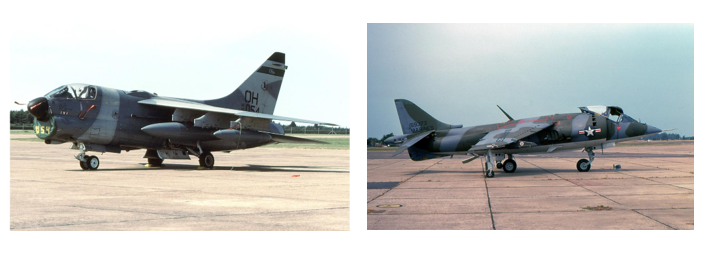
\includegraphics[scale=0.7]{obrazky-figures/a7dav8a.png}
\caption{Stíhacie letúny A-7D a AV-8A. Prevzaté z~\cite{fotoStihacky}.}{\label{stihacky}}
\end{figure}

\subsubsection{Aplikácie na pristátie za každého počasia}
Priehľadové displeje boli navrhnuté ako pomôcka na vyriešenie problémov, ktorým čelia piloti počas priblíženia na pristátie za nepriaznivých poveternostných podmienok. Lane a~Cumming študovali vizuálne podnety podniknuté pilotmi počas konečného priblíženia a~dospeli k~záveru, že vhodné vizuálne zameriavacie zariadenie by mohlo pomôcť pilotovi pri~posudzovaní činov pri~jeho priblížení. Počas vizuálneho priblíženia majú piloti problém letieť stabilizované priblíženie na bezpečnej zostupovej dráhe čo je zvyčajne rádovo tri stupne. Počas priblíženia pomocou prístrojov, letí pilot s~hlavou nadol zameranou na palubnú dosku. Pri dosiahnutí vizuálneho kontaktu, by mal pilot dokončiť pristátie vizuálne. Ak sú prítomné nejaké ilúzie, pilot môže byť týmito ilúziami privedený do omylu. Na problém má vplyv veľmi krátky časový interval medzi vizuálnym kontaktom a dotykom letúna s~pristávacou dráhou. Počas vizuálnych pristátiach by HUD mohol poskytovať vizuálne vedenie ako to opísal Gold \cite{4502188}. Tento typ HUD bol testovaný pri simulovaných nočných priblíženiach. HUD využívala spoločnosť Pacific Western Airlines, ktorá lietavala v~arktických podmienkach. Ako dôkaz toho, že displej môže byť cenný pri zlepšovaní bezpečnosti pri pristátiach bol ten, že bolo zaznamenaných trojnásobne menej nehôd pri pristávaní ako predtým \cite{HUDkniha}.

Počas fázy priblíženia pilot jednoducho lieta na HUD, akoby lietal podľa palubnej dosky. Umiestnenie letových údajov na čelné sklo by pomohlo prechodu na čisto vizuálny let, čo by pilotovi poskytlo viac času na posúdenie podnetov bez toho, aby sa vzdal týchto prístrojov. Tento typ HUD bol dôkladne testovaný v~Európe a taktiež aj v~USA \cite{HUDkniha}.

Začiatkom osemdesiatych rokov dvadsiateho storočia používal DC-9-80 neskôr nazývaný MD-80 podobnú koncepciu na monitorovanie priblíženia systému pristátia podľa prístrojov (ILS). Tento HUD prevádzkovali spoločnosti Swissair, Austrian Airlines a krátko nato aj Pacific Southwest Airlines \cite{HUDkniha}.

Pridanie systému syntetického videnie do HUD bolo navrhnuté ako ďalšia pomôcka pri~pristávaní za každého počasia. Systém syntetického videnia obsahuje plastické zobrazenie vonkajšieho terénu na tienitku HUD. Toto zobrazenie je vytvorené počítačom, na~základe získaných údajov o~letúne ako sú GPS poloha, kurz letúna, výška letúna. Americkej firme Chelton Flight Systems sa podarilo certifikovať systém elektronických letových prístrojov "Flight Logic", ktorý nahradil čiaru horizontu plastickým zobrazením okolného teréna. Tento systém bol dôkladne testovaný. Laboratóriom pre tento projekt bola Aljaška, ktorá je výnimočná svojím horským terénom a subarktickým podnebím. Na displeji je zobrazený 3D terén, kopce, vodné plochy, letiská. Vďaka SVS má pilot aj za horšej viditeľnosti neustály prehlad o~situáciach okolo letúna a môže tak zamedziť nebezpečnému zblíženiu s~terénom, než pri použití klasických navigačných prístrojov nachádzajúcich sa na panely.
Systémy syntetického videnia vyžadujú prísnejšiu certifikáciu ako systémy vylepšeného videnia (EVS). Na obrázku \ref{svs} môžete vidieť priehľadový displej, ktorý obsahuje systém syntetického videnia \cite{svs}.

\begin{figure}[ht]
\centering
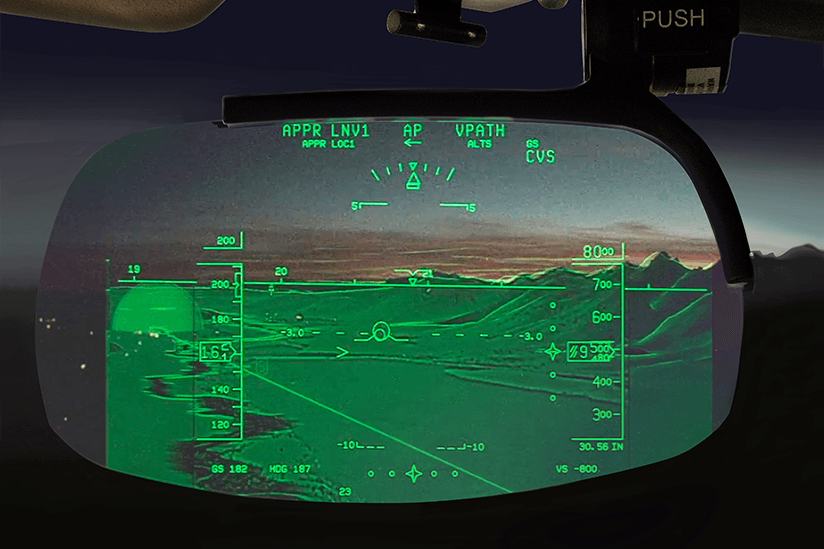
\includegraphics[scale=0.4]{obrazky-figures/SVS.png}
\caption{HUD so systémom syntetického videnia. Prevzaté z~\cite{fotoSv}.}{\label{svs}}
\end{figure}

\subsection{Priehľadový displej a priestorová dezorientácia}
V~skorých prieskumoch sa zistilo, že až 30\% pilotov lietajúcich na letúnoch vybavených BUD opisuje zvýšenú tendenciu k~priestorovej dezorientácii. Neskôr Newman a Foxworth zistili, že iba 14\% pilotov lietajúcich na stíhacom letúne F-18 vybavených HUD hlásili zvýšenú tendenciu k~SDO. HUD je jedná z~vecí, ktoré vyvolávajú SDO. Na priestorovú dezorientáciu majú vplyv aj extrémne manévre, ako je napríklad vzdušný bojový manéver (ACM). Účelom tohto manévra je ten, aby sa letún dostal do pozície, z~ktorej je možné zaútočiť na iný nepriateľský letún. Tyler a Furr popisujú medzi hlavné príčiny SDO znížené vizuálne podnety \cite{HUDkniha}.

HUD je obmedzený na monochromatické línie a musí sa vyhýbať textúram a vzorom, ktoré by mohli blokovať vonkajšie vizuálne podnety. Je nepravdepodobné, že displeje budú v~dohľadnej budúcnosti obsahovať farby s~dostatočným kontrastom. Bez ohľadu na technologický pokrok by nebolo praktické používať modrú farbu na označenie oblohy a hnedú farbu na označenie zeme. Modré symboly by neboli jasne viditeľné oproti skutočnej oblohe a hnedé symboly by dostatočne nekontrastovali s~niektorými terénmi. Namiesto farebného označenia boli použité iné veci, ako sú plné čiary nad horizontom a prerušované čiary pod~horizontom \cite{HUDkniha}.

HUD, ktoré sa používajú v~stíhacích letúnoch F-18 majú šikmé čiary sklonu vo veľkých uhloch na označenie smeru k~horizontu. Symbolika rýchleho prúdového letúna Royal Air Force (RAF) používa čiary sklonu, ktoré sa zdajú byť zužujúce sa a skracujú sa, keď sa uhol od horizontu zväčšuje. Štandard USAF kombinuje tieto dva prístupy a používa prerušované čiary sklonu pod horizontom a zúžené/plné čiary nad horizontom \cite{HUDkniha}.

Priehľadový displej v~stíhacom letúne F-16 bol považovaný ako rušivý a neprehľadný a~to kôli 2,5$^\circ$ rozstupu medzi čiaramy. Za neprehľadný displej sa považuje taktiež taký, ktorý obsahuje nadmerné množstvo informácií, čo predstavuje napríklad veľký počet rôznych symbolov alebo farieb \cite{HUDkniha}.

% Historia prehlad kniha koniec

\section{Letové prístroje letúna}
Letecké prístroje sú dané radou ciferníkov, meradiel a prístrojov nachádzajúcich sa v~kokpite letúna. Tieto prístroje slúžia pre pilotov ako pomôcka k~bezpečnému lietaniu. Prístroje ukazujú napríklad to, kde sa letún nachádza, akou rýchlosťou letí a taktiež mnoho ďalších informácií o~lete.
Existuju štyri základné druhy leteckých nástrojov, ktoré su zoradené podľa práce, ktorú vykonávajú. Sú to \cite{Instruments}:
\begin{itemize}
\item Stavové prístroje – sú prístroje, ktoré poskytujú informácie o~stave letúna (orientácia vzhľadom k~horizontálnej rovine).  Príklady sú napríklad výškomer, rýchlomer, smerový zotrvačník, umelý horizont, zatáčkomer a variometer.
\item Motorové prístroje – sú prístroje, ktoré merajú prevádzkové parametre motorov letúna. Príklady sú otáčkomer, ukazovateľ množstva paliva, ukazovateľ množstva oleja a ukazovateľ tlaku motora.
\item Navigačné prístroje – sú prístroje, ktoré poskytujú navádzacie informácie, ktoré umožňujú letúnu sledovať zamýšľanú dráhu. Príklady sú napríklad rôzne druhy navigačných zariadení, od jednoduchého kompasu a rádiolokácie až po GPS lokalizačné zariadenia.
\item Doplnkové prístroje – táto kategória zahŕňa rad rôznych meradiel a indikátorov, ktoré nie sú zahrnuté v~prvých troch kategóriach. Tieto prístroje poskytujú údaje o~polohách pohyblivých komponentov v~letúne a stave rôznych komponentov alebo systémov letúna. Príklady sú napríklad prostredie v~kabíne (tlak, teploty), polohy riadenia letu. 
\end{itemize}

\newpage
\subsection{Klasické rozmiestnenie letových prístrojov}
Je to balíček, obsahujúci 6 letových prístrojov, ktoré sa nachádzajú takmer v~každom letúne. Sú to \cite{Instruments}:
\begin{itemize}
    \item výškomer,
    \item rýchlomer,
    \item variometer,
    \item umelý horizont,
    \item smerový zotrvačník,
    \item zatáčkomer.
\end{itemize}

\subsubsection{Výškomer}
Výškomer zobrazuje aktuálnu nadmorskú výšku letúna. Mechanický výškomer obsahuje 3 ručičky, ktoré merajú stovky, tisíce a desaťtisíce stôp. Tieto ručičky sa pohybujú rôznymi rýchlosťami. Výslednú hodnotu výšky letúna dostaneme po spočítaní jednotlivých ručičiek~\cite{Instruments}. Na obrázku \ref{vyskomer} môžete vidieť mechanický výškomer skladajúci sa z~3 ručičiek.
\begin{figure}[ht]
\centering
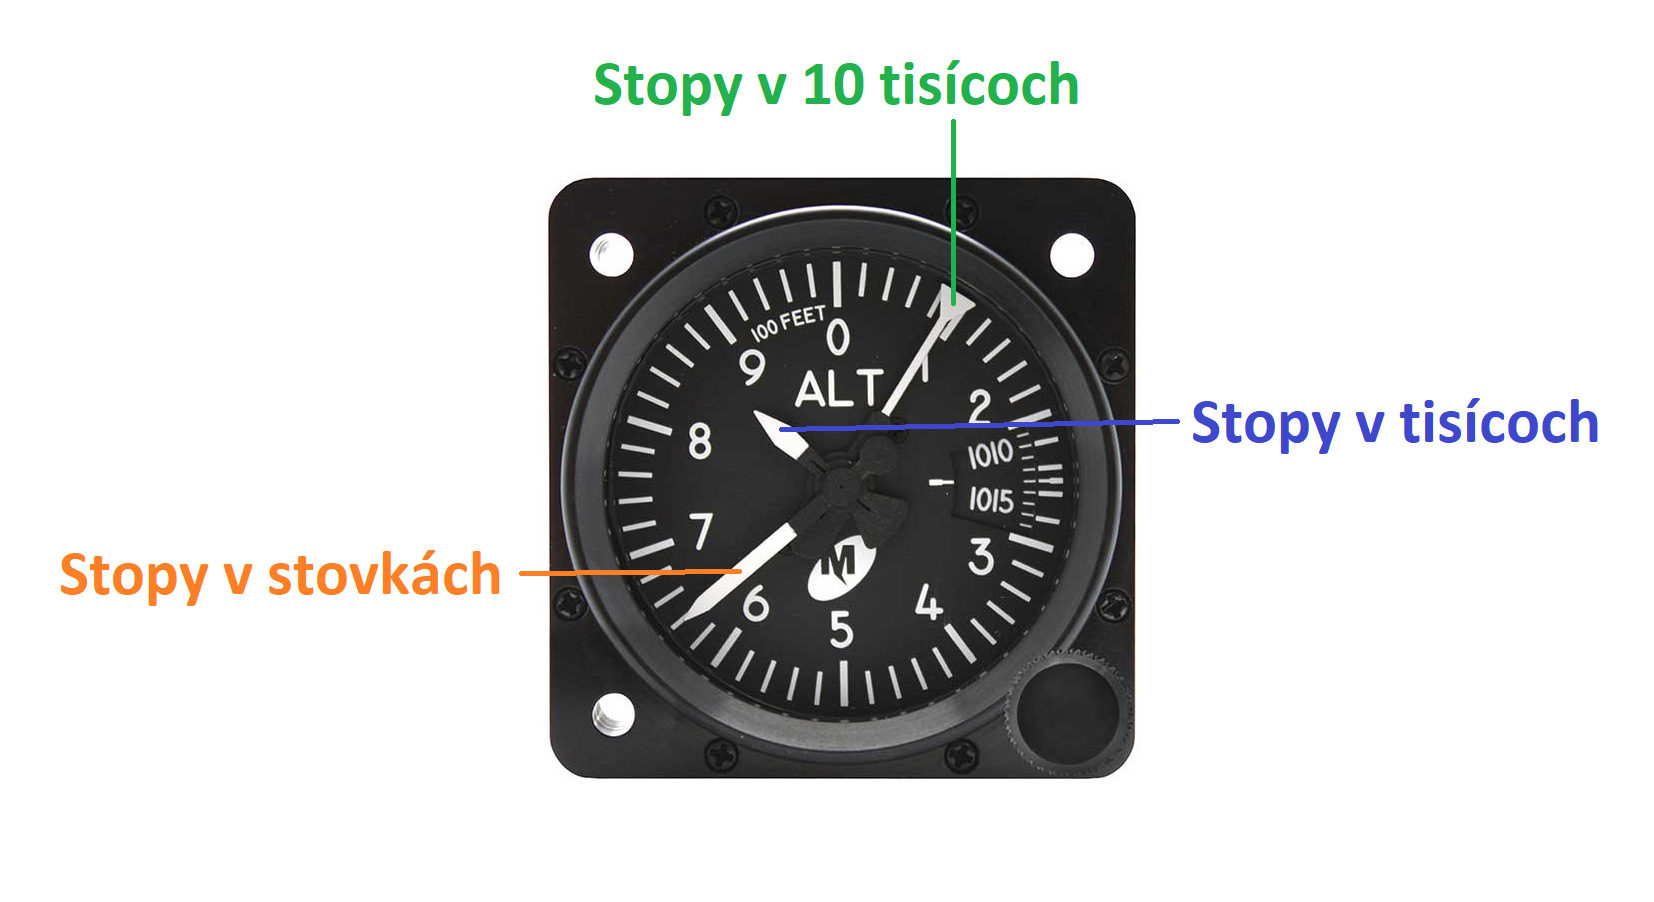
\includegraphics[height=7cm, width=13cm]{obrazky-figures/vyskomer.png}
\caption{Mechanický výškomer. Prevzaté z~\cite{fotoIndikator}.}{\label{vyskomer}}
\end{figure}


%\bigskip
Existuje 5 typov nadmorských výšok. Sú to \cite{Altitude}:
\begin{itemize}
    \item Indikovaná nadmorská výška – je nadmorská výška uvedená na výškomere, pri nastavenom barometrickom tlaku. Jednoducho povedané, je to nadmorská výška, ktorú priamo odčítame z~výškomeru. 
    \item Skutočná nadmorská výška – je vertikálna vzdialenosť letúna nad hladinou mora (MSL). Udáva nadmorskú výšku upravenú o~neštandardnú teplotu a tlak.
    \item Absolútna nadmorská výška – je výška, ktorá sa neustále mení. Absolútna výška je výška nad úrovňou terénu (AGL). Radarový výškomer meria nadmorskú výšku nad terénom, ktorý sa momentálne nachádza pod letúnom. Radarové výškomery vo~všeobecnosti poskytujú informačné údaje až do 2500 stôp AGL.
    \item Tlaková nadmorská výška – je nadmorská výška, uvedená na výškomere na základe štandardnej atmosferickej hladiny. Tlaková výška sa primárne používa pri výpočtoch výkonu letúna a pri lete vo veľkých výškach. 
    \item Hustota nadmorskej výšky – je tlaková nadmorská výška, upravená o~teplotu. Ovplyvňuje výkonové parametre každého letúna. Čím vyššia je hustota nadmorskej výšky, tým nižší je výkon letúna a naopak.
\end{itemize}

\subsubsection{Princíp fungovania výškomeru}
Hodnoty výškomera závisia na barometrickom tlaku. Vzhľadom k~tomu, že sa barometrický tlak neustále mení, je potrebné výškomer nastaviť pred a taktiež počas každého letu.

Výškomer funguje tak, že sa využíva statický port na vonkajšej strane letúna. Pri zmene nadmorskej výšky spôsobuje, že sa aneroid rozťahuje a sťahuje, čo spôsobuje zmenu údaja na~meradle. Tieto informácie sa používajú v~spojení s~prednastaveným barometrickým tlakom na poskytnutie odčítania nadmorskej výšky \cite{Instruments}.

\bigskip
\subsubsection{Rýchlomer}
Tento indikátor meria rýchlosť letúna pri jeho lete pomocou rozdielov tlaku vzduchu zo~statického portu a z~pitotovej trubice. Tento rozdiel v~tlaku sa zaznamenáva pomocou ukazovateľa ASI na prednej strane prístroja. Mechanické ASI sa skladá z~rastúcich čísel nachádzajúcich sa na okrúhlom ciferníku s~jednou ručičkou, ktorá ukazuje aktuálnu rýchlosť letúna. Toto meranie sa najčastejšie uvádza v~uzloch čo sú námorné míle za hodinu, ale taktiež sa môžu uvádzať aj v~iných formátoch, ako sú napríklad kilometre za hodinu \cite{Instruments}. Na obrázku \ref{ASI} môžete vidieť mechanický rýchlomer skladajúci sa z~jednej ručičky udávajúc aktuálnu rýchlosť.
\begin{figure}[ht]
\centering
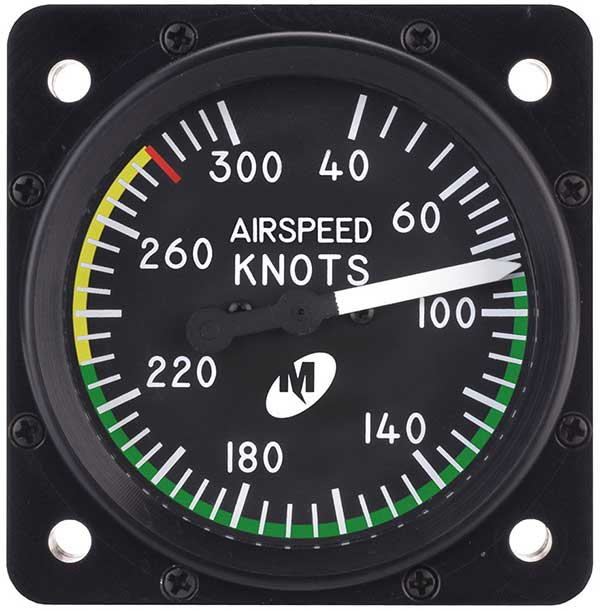
\includegraphics[height=5cm, width=5cm]{obrazky-figures/rychlomer.png}
\caption{Mechanický rýchlomer. Prevzaté z~\cite{fotoIndikator}.}{\label{ASI}}
\end{figure}

Existujú 4 typy rýchlostí letúna. Sú to \cite{Airspeed}:
\begin{itemize}
    \item Indikovaná rýchlosť (IAS) – je rýchlosť bez ohľadu na atmosferické podmienky. Tento typ rýchlosti sa používa na to, aby výrobcom poskytovala odporúčania pre výkonové údaje letúna týkajúce sa rýchlosti vzletu, pristátia a pádu. Pri stúpaní letúna hustota vzduchu klesá a indikovaná rýchlosť bude nižšia, ako skutočná rýchlosť vzduchu (TAS). Pri riadení letúna je indikovaná rýchlosť dôležitejšia, ako skutočná rýchlosť~\cite{Indicated}. 
    \item Kalibrovaná rýchlosť (CAS) – je indikovaná rýchlosť opravená pre chyby prístroja a~chybu polohy. CAS má dve primárne aplikácie v~letectve \cite{Calibrated}:
    \begin{enumerate}
        \item Pre navigáciu sa CAS počíta ako jeden z~krokov medzi indikovanou vzdušnou rýchlosťou a skutočnou vzdušnou rýchlosťou.
        \item Pre riadenie letúna je CAS jeden z~primárnych referenčných bodov, pretože popisuje dynamický tlak pôsobiaci na povrch letúna bez ohľadu na existujúce podmienky teploty, tlakovej výšky alebo vetra.
    \end{enumerate}
    \item Skutočná rýchlosť (TAS) – je rýchlosť letúna vzhľadom na vzduch, cez ktorý prechádza. Letúny s~prúdovými motormi dokážu dosiahnúť práve túto vyššiu rýchlosť vo vysokých nadmorských výškach na základe toho, že ich motory sú vo vysokých nadmorských výškach efektívnejšie \cite{Airspeed}.
    \item Pozemná rýchlosť (GS) – je aktuálna rýchlosť letúna nad zemou alebo skutočná rýchlosť letúna upravená pre faktory rýchlosti vetra, ako napríklad protivietor alebo zadný vietor.
\end{itemize}

\bigskip
\subsubsection{Variometer}
Jeho funkciou je zobrazovať rýchlosť stúpania alebo klesania v~stovkách stôp za minútu. Pomocou pitot-statického systému dokáže zhromažďovať svoje merania. Taktiež je známy pod označovaním, ako indikátor rýchlosti stúpania.

Variometer nie je na pohľad zložitý, dá sa ľahko pochopiť, ako funguje. Skladá sa zo~šiestich častí, ktoré zabezpečujú funkčnosť indikátora. Sú to \cite{vsiAirspeed}:
\begin{itemize}
    \item Port statického tlaku – otvor nachádzajúci sa na vonkajšej strane letúna. Jeho úlohou je zachytávať okolitý vzduch a smerovať ho do statického vedenia.
    \item Statické vedenie – skladá sa z~dutej trubice, ktorá spája port statického tlaku s~púzdrom a membránou variometra.
    \item Púzdro – obsahuje ostatné komponenty ukazovateľa vertikálnej rýchlosti. Toto púzdro je pripojené k~statickému vedeniu pomocou spojenia s~kalibrovanou časťou.
    \item Kalibrovanú časť pre únik – je špeciálny typ spojenia medzi púzdrom a statickým vedením. Táto časť pri prúdení vzduchu do púzdra zabraňuje okamžitej zmene tlaku vo vnútri púzdra.
    \item Membránu – je to flexibilná kovová nádoba, ktorá sa nachádza sa vo vnútri púzdra a~je pripojená priamo k~statickému vedeniu. 
    \item Čelná strana – je to predná časť indikátora, ktorá je viditeľná v~kabíne letúna. Z~tejto obrazovky dokáže pilot získať údaje o~vertikálnej rýchlosti letúna. Samotná ihla nachádzajúca sa na čelnej strane je pripojená k~membráne pomocou ozubených kolies a~tyčí.
\end{itemize}
Na obrázku \ref{VSI} môžete vidieť variometer letúna.
\begin{figure}[ht]
\centering
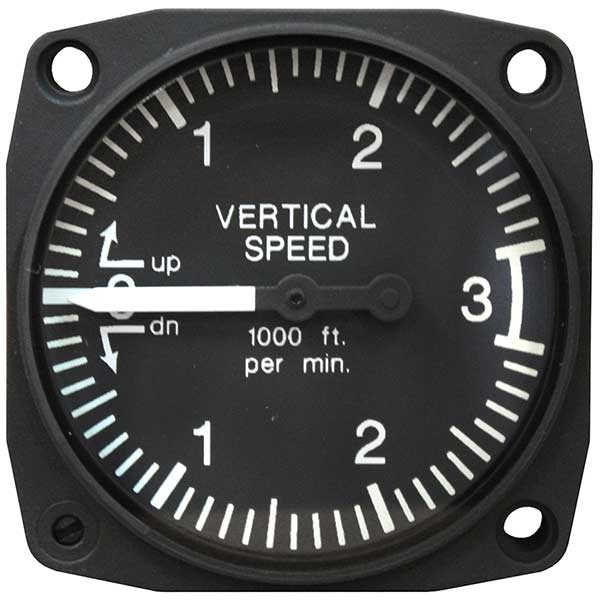
\includegraphics[height=5cm, width=5cm]{obrazky-figures/variometer.png}
\caption{Mechanický variometer. Prevzaté z~\cite{fotoIndikator}.}{\label{VSI}}
\end{figure}
\newpage
\bigskip
\subsubsection{Umelý horizont}
História siaha k~začiatkom 20. storočia kde v~roku 1916 Lawrence Sperry testoval umelý horizont. V~roku 1929 letec Jimmy Doolittle uskutočnil prvý let podľa prístrojov, kde vykonal vzlet a pristátie pomocou umelého horizontu Sperry. Počas vojny boli umelé horizonty bežnou súčasťou vo vojenských letúnoch. V~súčasnosti sa umelé horizonty nachádzajú takmer vo všetkých letúnoch \cite{gyroscopeHistory}.

Jeho ovládacím mechanizmom je malé koliesko s~vertikálnou osou otáčania, roztáčané prúdom vzduchu alebo elektromotorom. Horná polovica číselníka je modrej farby a predstavuje oblohu. Dolná polovica číselníka je hnedej farby a predstavuje zem. Na obrázku \ref{poloha} je znázornený klasický umelý horizont. Slúži na to aby pilotovi poskytol informácie o~relatívnej polohe letúna k~zemskému horizontu. Vďaka číselníku, ktorý sa nachádza v~kokpite letúna pilot má informácie o~tom, či letún stúpa, klesá alebo sa nakláňa. Mechanické gyroskopové indikátory sa stále používajú v~mnohých letúnoch. V~súčasnosti sú známejšie už elektrické a digitálne verzie \cite{gyroscope}.


\begin{figure}[ht]
\centering
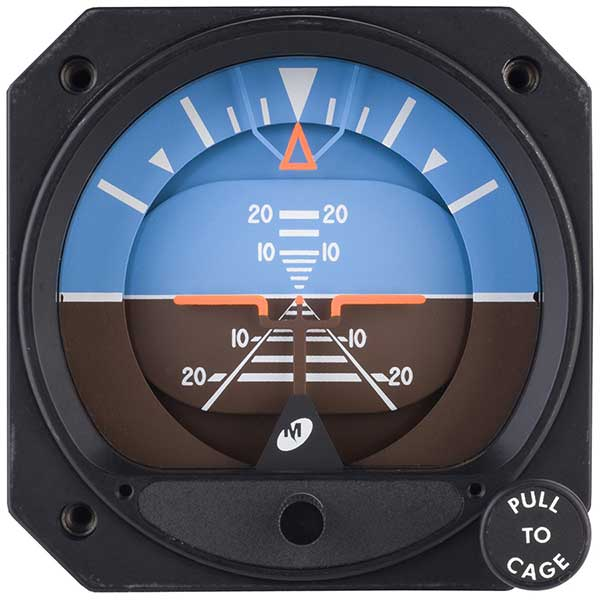
\includegraphics[height=5cm, width=5cm]{obrazky-figures/umelyhorizont.png}
\caption{Mechanický umelý horizont. Prevzaté z~\cite{fotoIndikator}.}{\label{poloha}}
\end{figure}

\bigskip
\subsubsection{Smerový zotrvačník}
Je prístroj, určený na informovanie pilota o~tom, ktorým smerom letún smeruje. Smerový zotrvačník je pokrokom oproti používaniu magnetického kompasu. Používanie magnetického kompasu môže mať nevýhodu, a to takú, že pri turbulentnom lete to sťažuje dosiahnutie priameho letu a dodržanie presného smeru. Smerový zotrvačník na rozdiel od magnetického kompasu nie je ovplyvnený týmito silami \cite{gyroscopeHeading}. Poskytuje zvýšenú presnosť, lepšiu spoľahlivosť a ľahko čitateľný ciferník, ktorý predstavuje sever, juh, východ a západ pomocou 360$^\circ$ kompasu. Na obrázku \ref{heading} je znázornený mechanický smerový zotrvačník.

Existuje viacero typov ukazovateľov s~rôznym stupňom presnosti. Siahajú od základných indikátorov, ktoré sú poháňané vákuom až po indikátory, ktoré obsahujú podporu GPS. Pri jednoduchom indikátore je nutné opätovné nastavenie každých 10 až 20 minút, zatiaľ čo sofistikované zariadenia, ako sú indikátory, ktoré sa nachádzajú v~prúdových letúnoch, využívajú presnú laserovú technológiu \cite{heading}.

\begin{figure}[ht]
\centering
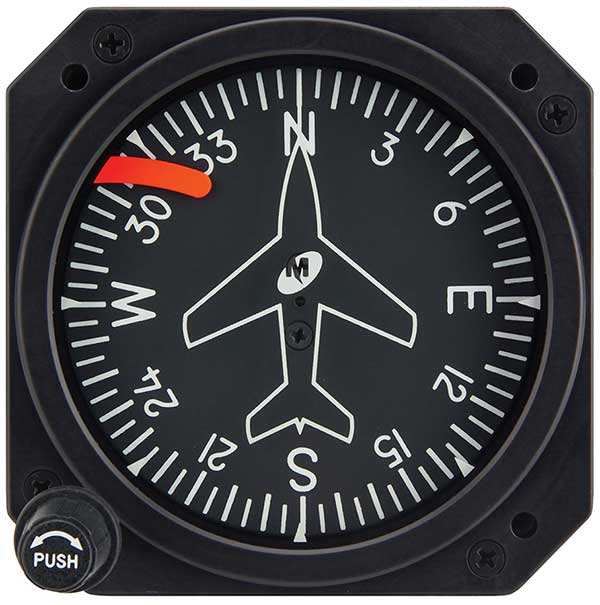
\includegraphics[height=5cm, width=5cm]{obrazky-figures/smerovyzotrvacnik.png}
\caption{Mechanický smerový zotrvačník. Prevzaté z~\cite{fotoIndikator}.}{\label{heading}}
\end{figure}

\bigskip
\subsubsection{Zatáčkomer}
Je nástroj, ktorý dokáže snímať pohyby náklonu aj zatáčania. Tieto pohyby zobrazuje na~základe dvoch komponentov, ktoré obsahuje. Prvá je ihla, ktorá má tvar letúna a plní funkciu otáčania sa doprava alebo doľava. Druhá komponenta je sklonomer, ktorý má tvar čiernej gule zavesenej na kvapaline, ktorá sa nachádza v~strede a taktiež sa pohybuje doprava alebo doľava. Označenie 2 MIN na koordinátore značí to, že ak sa letún otáča rýchlosťou 3 stupne za sekundu tak vykonáte obrat o~360 stupňov za dve minúty \cite{turn}. Na obrázku \ref{turning} je znázornený zatáčkomer letúna.

\begin{figure}[ht]
\centering
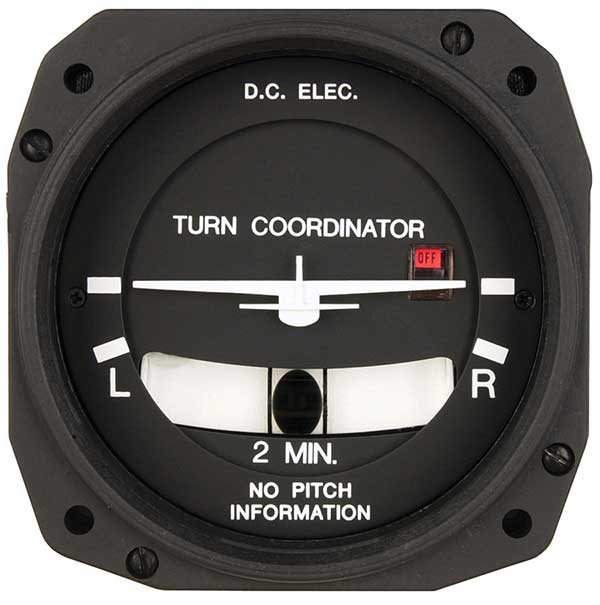
\includegraphics[height=5cm, width=5cm]{obrazky-figures/zatackomer.png}
\caption{Mechanický zatáčkomer. Prevzaté z~\cite{fotoIndikator}.}{\label{turning}}
\end{figure}

%\label{zaverPrace}

%----------------------------SUCASNOST-----------------------------------
\chapter{Súčasné trendy vizualizácie letových dát}
Na úvod je v~tejto kapilote spomenutý head down display (HDD). V~tejto kapitole bude popísaný následne head-up displej. Následne budú spomenuté výhody, ktoré ponúka pilotom pre jednoduchšie a bezpečnejšie lietanie. Taktiež sú tu spomenuté štatistické údaje, ktoré súvisia s~HUD a funkcie, ktoré najnovšie displeje poskytujú. V~kapitole sú spomenuté tri generácie displejov a popísaná symbolika HUD. Na konci kapitoli je popísaný HMD a taktiež výhody ktoré nám ponúka.

\section{Head Down Display}
Do tejto kategórie (HDD) zaraďujeme dva typy displejov. Prvý je prímárny letový displej (PFD) a druhý je multifunkčný displej (MFD).

\subsection{Primány letový displej}
Primárny letový displej (PFD), ktorý sa nachádza v~letúne vybavenom elektronickým letovým prístrojovým systémom, je primárnou referenciou pilota pre letové informácie. Jednotka kombinuje informácie zobrazované na niekoľkých elektromechanických prístrojoch do jedného elektronického displeja, čím sa znižuje pracovné zaťaženie pilota a zvyšuje sa informovanosť o~situácii \cite{pfd}.

Rozloženie a informácie zobrazené na PFD sa líšia v~závislosti od výrobcu a inštalácie. Väčšina primárnych letových displejov je nakonfigurovaná s~centrálnym ukazovateľom polohy (AI) a flight director obklopeným inými letovými parametrami. Konvencia zvyčajne umiestňuje pásku rýchlosti letu na ľavú stranu AI a referencie nadmorskej výšky a vertikálnej rýchlosti na pravú. Vertikálna odchýlka pre zostup ILS alebo vertikálnu navigáciu (VNAV) sa zobrazuje napravo od AI, zatiaľ čo bočná odchýlka od dráhy ILS, VOR alebo FMS sa zobrazuje pod AI. V~spodnej časti prístroja sa nachádza referencia kompasu, zataľ čo vo väčšine prípadov sú režimy priblíženia, autopilota signalizované na hornej časti prístroja. Primárny letový displej je znázornený na obrázku \ref{PFD} \cite{pfd}.

\begin{figure}[ht]
\centering
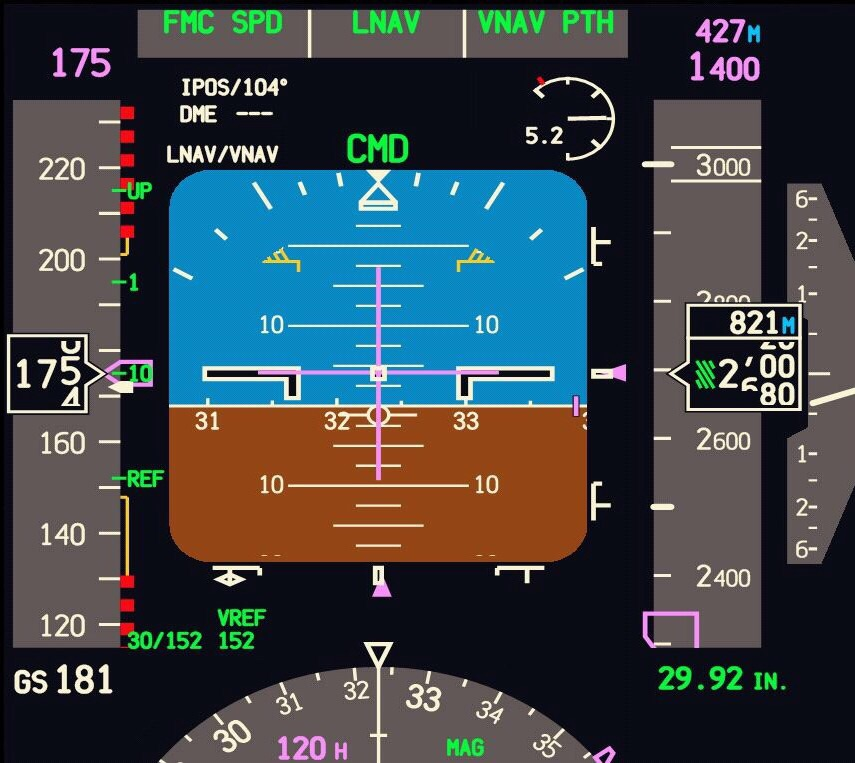
\includegraphics[scale=0.25]{obrazky-figures/PFD.png}
\caption{Primárny letový displej. Prevzaté z~\cite{fotoPFD}.}{\label{PFD}}
\end{figure}
\newpage

\subsection{Multifunkčný displej}
Základom funkčnosti multifunkčného displeja (MFD) je schopnosť súčasne prezentovať informácie z~rôznych zdrojov pomocou prekrytiaobrazovky a okien. Aj keď je táto funkcia užitočná na integráciu údajov z~rôznych zdrojov, vytvára tiež potenciál pre neporiadok na~displeji. Ovládače MFD by mali byť ľahko prístupné a vhodne umiestnené, aby umožňovali jednoduchú obsluhu. Ovládacie prvky by mali byť priestorovo oddelené a ovládacie prvky, ktoré sa ovládajú počas letu, by mali byť viditeľné za akýchkoľvek svetelných podmienok. Ovládače MFD podporujú zadávanie údajov. Systém by mal toto zadávanie uľahčovať a umožňovať viac ako jeden spôsob vkladania údajov. Mal by byť navrhnutý tak, aby pomohol predchádzať závažným chybám pri zadávaní údajov. Schopnosť pohybovať sa medzi viacerými obrazovkami, stránkami a oknami je dôležitým aspektom rozhrania. Taktiež je dôležité, aby používateľ mohol rýchlo a jednoducho prepínať madzi hlavnými funkciami displeja, ktoré systém poskytuje. K~dispozícii je niekoľko spôsobov ovládania MFD. Výber môže prebiehať buď priamo pomocou tlačidiel alebo dotykovej obrazovky alebo nepriamo pomocou klávesnice alebo joysticku. Bez ohľadu na metódy vstupu ovládania, výber možností na displejoch MFD sa musí vykonávať stabilne a jednoducho.

Menu MFD by malo byť organizované tak, aby dávalo pilotovi zmysel. Optimálna organizácia ponuky a zobrazenia je založená na funkčných kategóriach, ako sú systémy letúna, počasie, premávka, terén či komunikácia. Aby sa zachovala účinnosť, použitie farieb by malo byť konzistentné v~celom MFD. Farby môžu byť veľmi účinné a uľahčiť spracovanie informácií z~elektronických displejov. Aby bolo použitie farieb v~MFD efektívne, farby musia byť zreteľné a zmysluplné. Multifunkčný displej je znázornený na obrázku \ref{MFD} \cite{MFD}.

\begin{figure}[ht]
\centering
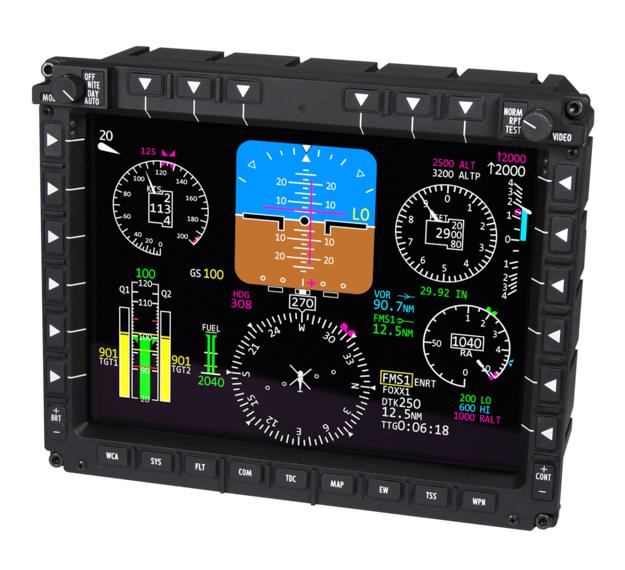
\includegraphics[scale=0.35]{obrazky-figures/MFD.png}
\caption{Multifunkčný displej. Prevzaté z~\cite{fotoMFD}.}{\label{MFD}}
\end{figure}
\newpage

\section{Head Up Display}
%V súčasnosti nie je priehľadový displej (HUD) žiadnou novinkou.
V~letectve sa head-up displeje používajú už desaťročia a to hlavne vojenskými pilotmi. V~dnešnej dobe sú head-up displeje bežnou súčasťou veľkých komerčných letúnov a taktiež aj súkromných letúnov. Displej zobrazuje všetky potrebné údaje o~navigácií a lete na obrazovke, ktorá sa nachádza v~úrovni očí pilota, takže nemusia spúšťať zrak od okolitého okolia a nemusia pozerať na~svoje prístroje. Vďaka holografickým technológiám vyzerá obraz tak, akoby bol vzdialený ďaleko pred letúnom, a pritom môže byť vzdialený iba pár centimetrov od pilota \cite{SafetyHUD}. Je~potvrdené, že head-up displej znižuje pracovné zaťaženie pilotov, čo zvyšuje bezpečnosť a~znižuje nehodovosť.

Priehľadové displeje môžu byť užitočné hlavne počas pristátia alebo počas vzletu. Tieto fázy letu patria medzi najnebezpečnejšie. Pri pristávaní dokáže byť HUD nápomocný v~tom, že môže zohľadniť faktory, ako je bočný vietor a dokáže navrhnúť ideálnu trajektóriu pre~pristátie, ktorú bude pilot sledovať. Taktiež dokáže pilotovi pomôcť pri horších podmienkach prostredia, ako je napríklad hmlisté počasie \cite{HUDnight}.

Štúdia FSF sa zamerala na dopravne nehody v~minulosti v~rokoch 1959 až 1989 a zistili, že z~1079 dopravných nehôd civilných prúdových letúnov, ktoré nevyužívali HUD by pri~jeho využívaní mohlo zabrániť alebo pozitívne ovplyvniť 33\% nehôd s~úplnými stratami životov a 29\% nehôd s~veľkými stratami životov. Aktuálna mapa globálnej bezpečnosti letectva zahŕňa HUD v~odporúčaniach na lepšie využitie technológie pre zvýšenie bezpečnosti prevádzky letúnov počas priblíženia a pristátia \cite{SafetyHUD}.

\subsection{Komponenty priehľadového displeja}
Pre správne a efektívne fungovanie HUD je potrebné aby systém obsahoval následujúce komponenty \cite{HUDkomponenty}:
\begin{itemize}
    \item Počítač, ktorý prijíma údaje zo senzorov letúna, prístrojov a satelitných údajov.
    \item Priehľadná obrazovka (tienitko), ktorá je vyrobená zo skla alebo z~plastu. Obrazovka odráža informácie, ktoré pilot môže sledovať bez toho, aby mu bránila vo výhľade cez~čelné sklo alebo taktiež, aby blokovala priechod okolitého svetla.
    \item Ovládací panel, ktorý umožňuje pilotovi výber z~rôznych možností zobrazenia a údajov, ktoré sa majú zobraziť.
    \item Projektor, ktorý premieta získané údaje na tienitko. Moderné systémy HUD odstránili jednotky projektora a namiesto toho sú schopné generovať údaje priamo na obrazovku.
\end{itemize}

\subsection{Generácie priehľadového displeja}
Pri vývoji HUD vznikli tri základné generácie displejov. Jednotlivé generácie sa od seba líška rôznymi typmi displejov. V~každej generácií existujú ako výhody tak aj nevýhody.
\subsubsection{Prvá generácia}
HUD prvej generácie využívali displej s~katódovou trubicou (CRT) pre vytváranie obrazov na vrstve fosforu nachádzajúceho sa na obrazovke. CRT vytvára obrazy generovaním elektrónových lúčov, ktoré dopadajú na čelo trubice, ktorá je pokryta fosforom. Fosfory vydávajú svetlo, keď elektróny dopadnú. Lúč je zaostrený cievkami v~blízkosti katódového zdroja. Intenzita lúča určuje, aký jasný bude obraz. Pre danú trubicu, rýchlosť, ktorou sa škvrna pohybuje, určuje jas symbolu. Čím rýchlejší je pohyb, tým je symbol menej jasný. Typicky sú symboly alebo obrázky prekreslené päťdesiat alebo šesťdesiat krát za sekundu. Ak by obnovovacia frekvencia bola nižšia ako päťdesiat krát za sekundu, potom by to mohlo spôsobiť to, že by obraz mohol blikať alebo skákať. V~opačnom prípade, keby bola obnovovacia frekvencia väčšia ako šesťdesiat krát za sekundu tak by to mohlo spôsobiť, že by obraz nebol dostatočne jasný. Ak by do symboliky bolo začlenených príliš veľa symbolov, tak nebude dostatok času na ich vygenerovanie počas jedného obnovenia. Katódová trúbica je poháňaná generátorom symbolov. Generátor symbolov berie vstupné údaje z~počítača a prevádza ich na zmysluplnú symboliku, aby odovzdal informácie pilotovi. Niektoré priehľadové displeje spájajú funkcie generátora symbolov a počítača do jednej čiernej skrinky. Mnohé HUD využívajúce CRT displeje sa používajú dodnes avšak fosforová vrstva obrazovky sa časom opotrebováva. Takýto HUD môžete vidieť na obrázku \ref{hudSRT} \cite{HUDkniha}.

V~rastrovej symbolike môže generátor symbolov produkovať obraz vo formáte videa zloženého z~rastrového obrazu. Rastrový obrázok prechádza cez plochu CRT v~štandardnom vzore rovnobežných línií a potom sa vracia do východiskového bodu rýchlym pohybom nazývaným spätný chod. Pri tomto type zobrazenia sú stopy \textit{x(t)} a \textit{y(t)} vopred určené a~intenzita \textit{z(t)} sa používa na vytvorenie vzoru zobrazujúceho obraz. Obraz sa skladá zo~série pixelov sledujúcich stopu čiar \cite{HUDkniha}.

Niektoré skoršie priehľadové displeje vytvárali pohyblivé obrázky pomocou elektromechanických pohybov meračov, ktoré boli osvetlené alebo ktoré odrážali svetelné lúče. Keďže viaceré pohyby merača sa navzájom rušia, tento typ zdroja obrazu bol dosť obmedzený v~počte symbolov, ktoré bolo možné zobraziť. Elektromechanický zdroj symbolov má jednu výhodu. Odkedy symbol vzniká fyzickým pohybom drôtu, je možné sledovať jeho umiestnenie. To môže poskytnúť priame sledovanie zobrazovaných údajov. Tento typ zdroja obrazu sa už nevyrába \cite{HUDkniha}.

\begin{figure}[ht]
\centering
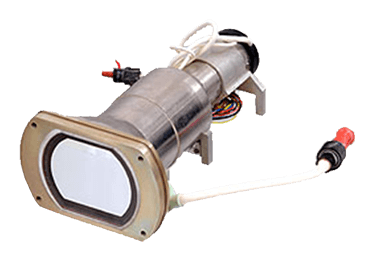
\includegraphics[scale=0.7]{obrazky-figures/HUD_SRT.png}
\caption{Technológia CRT vyvinutá spoločnosťou \textsc{Thomas Electronics}$^{\circledR}$. Prevzaté z~\cite{fotoCRT}.}{\label{hudSRT}}
\end{figure}

\subsubsection{Druhá generácia}
Druhá generácia HUD zaviedla používanie polovodičových svetelných zdrojov, ako sú diódy vyžarujúce svetlo (LED), modulované obrazovkou LCD na zobrazenie obrazov. Svetelné diódy LED sa pre HUD nepoužívali z~dôvodu obmedzeného jasu. Ak by bolo možné dosiahnúť dostatočného jasu, znížené požiadavky na výkon a veľkosť LED by ich urobili atraktívnymi. LED displeje musia mapovať symboly na pole pixelov \cite{HUDkniha}.

Tieto systémy po čase nedegradujú obraz a taktiež nie je potreba výsokého napätia. V~súčasnosti mnoho komerčných letúnov používa práve tento typ HUD \cite{HUDkomponenty}.

\subsubsection{Tretia generácia}
V~tretej generácií využívajú HUD optické vlnovody, ktoré vytvárajú obraz priamo v~zlučovači, bez potreby projekčného systému. Jeho nevýhoda je tá, že je viditeľný iba z~určitého uhla pohľadu, takže pilot má obmedzený priestor na pohyb hlavy. Niektoré z~najnovších systémov HUD využívajú skenovací laser, ktorý dokáže zobrazovať obrázky a videá na čírom transparentnom médiu, ako je napríklad čelné sklo letúna. Výrobcovia HUD začínajú pracovať so zobrazovacími technológiami, ako sú tekuté kryštály na kremíku, digitálne mikro zrkadlá a organické diódy vyžarujúce svetlo (OLED) za účelom znížiť veľkosť, hmotnosť a~zložitosť systémov HUD \cite{HUDkomponenty}. Podobne ako displeje v~druhej generácii sa displeje v~tretej generácií s~tekutými kryštálmi (LCD) nepoužívali z~dôvodu obmedzeného jasu. LCD displeje taktiež musia mapovať symboly na pole pixelov. Na obrázku \ref{lcdHUD} je znázornená štruktúra displeja z~tekutých kryštálov. Popis jednotlivých vrstiev \cite{LCDdisplej}:

\begin{enumerate}
    \item Vertikálny filtračný film na polarizáciu svetla pri vstupe.
    \item Sklenený substrát s~elektródami z~oxidu india a cínu (ITO). Tvary týchto elektród určia tvary, ktoré sa objavia po zapnutí LCD.
    \item Točené nematické tekuté kryštály.
    \item Sklenený substrát s~bežným elektródovým filmom (ITO) s~vodorovnými ryhami na~vyrovnanie s~horizontálnym filtrom.
    \item Horizontálna filtračná fólia na blokovanie/prepúštanie svetla.
    \item Reflexný povrch na posielanie svetla späť k~pozorovateľovi. 
\end{enumerate}

\begin{figure}[ht]
\centering
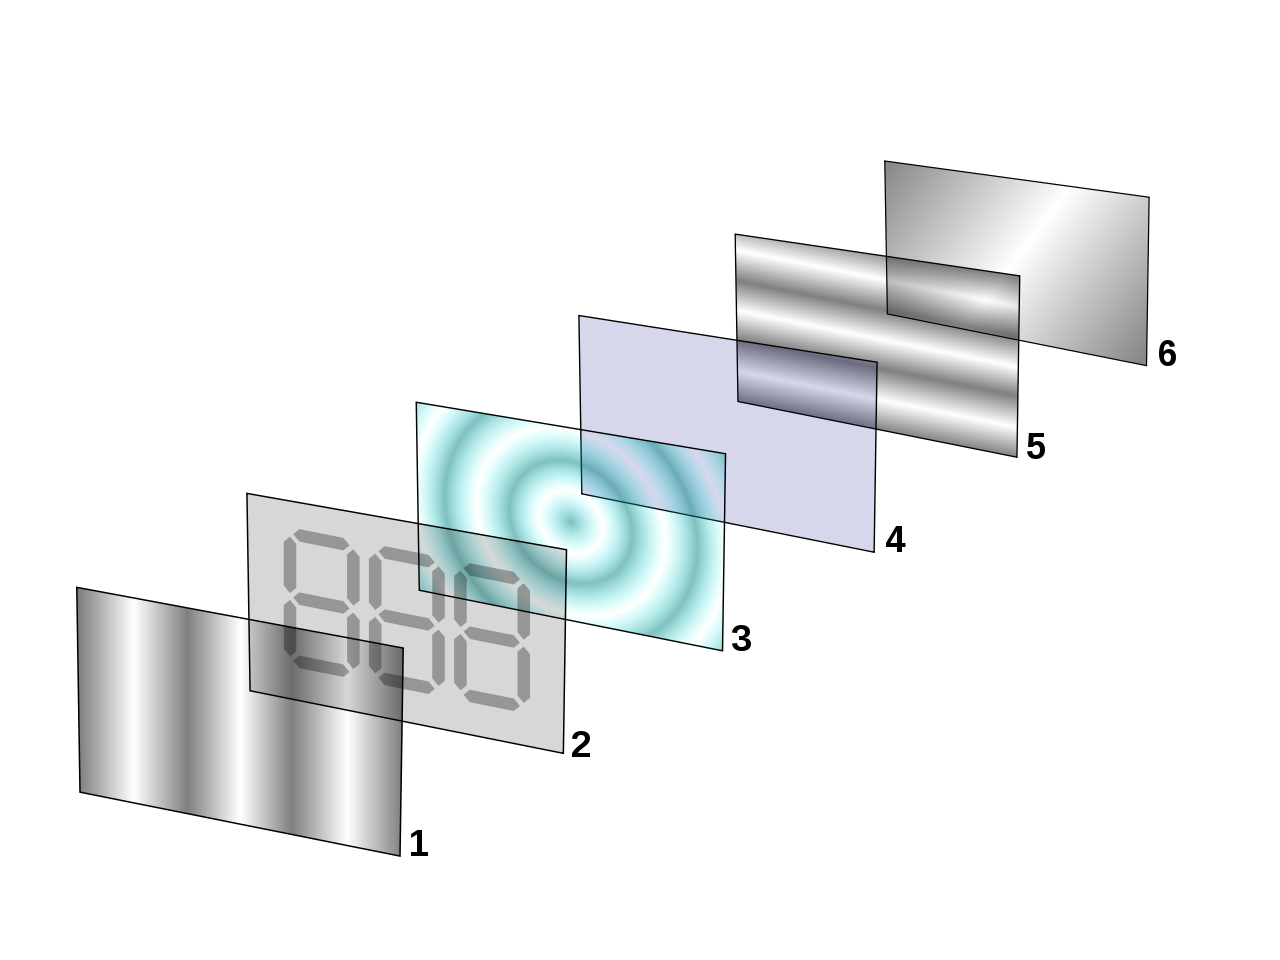
\includegraphics[scale=0.23]{obrazky-figures/LCDdisplay.png}
\caption{Vrstvy displeja z~tekutých kryštálov. Prevzaté z~\cite{fotoLCD}.}{\label{lcdHUD}}
\end{figure}

\subsection{Stav súčasných priehľadových displejov v~letectve}
Súčasné displeje sa líšia oproti tým, čo boli v~minulosti. Najnovšie HUD v~letúnoch zahrňujú~\cite{HUDnight}:
\begin{itemize}
    \item Viac zobrazovacej plochy. Napríklad Boeing sa rozhodol pri modely Dreamliner 787 vytvoriť dva panely HUD. Tieto panely majú viac, ako dvojnásobnú veľkosť zobrazovacej plochy oproti modelu Boeing 777. Tento HUD môžete vidieť na obrázku \ref{787hud}.
    \begin{figure}[ht]
\centering
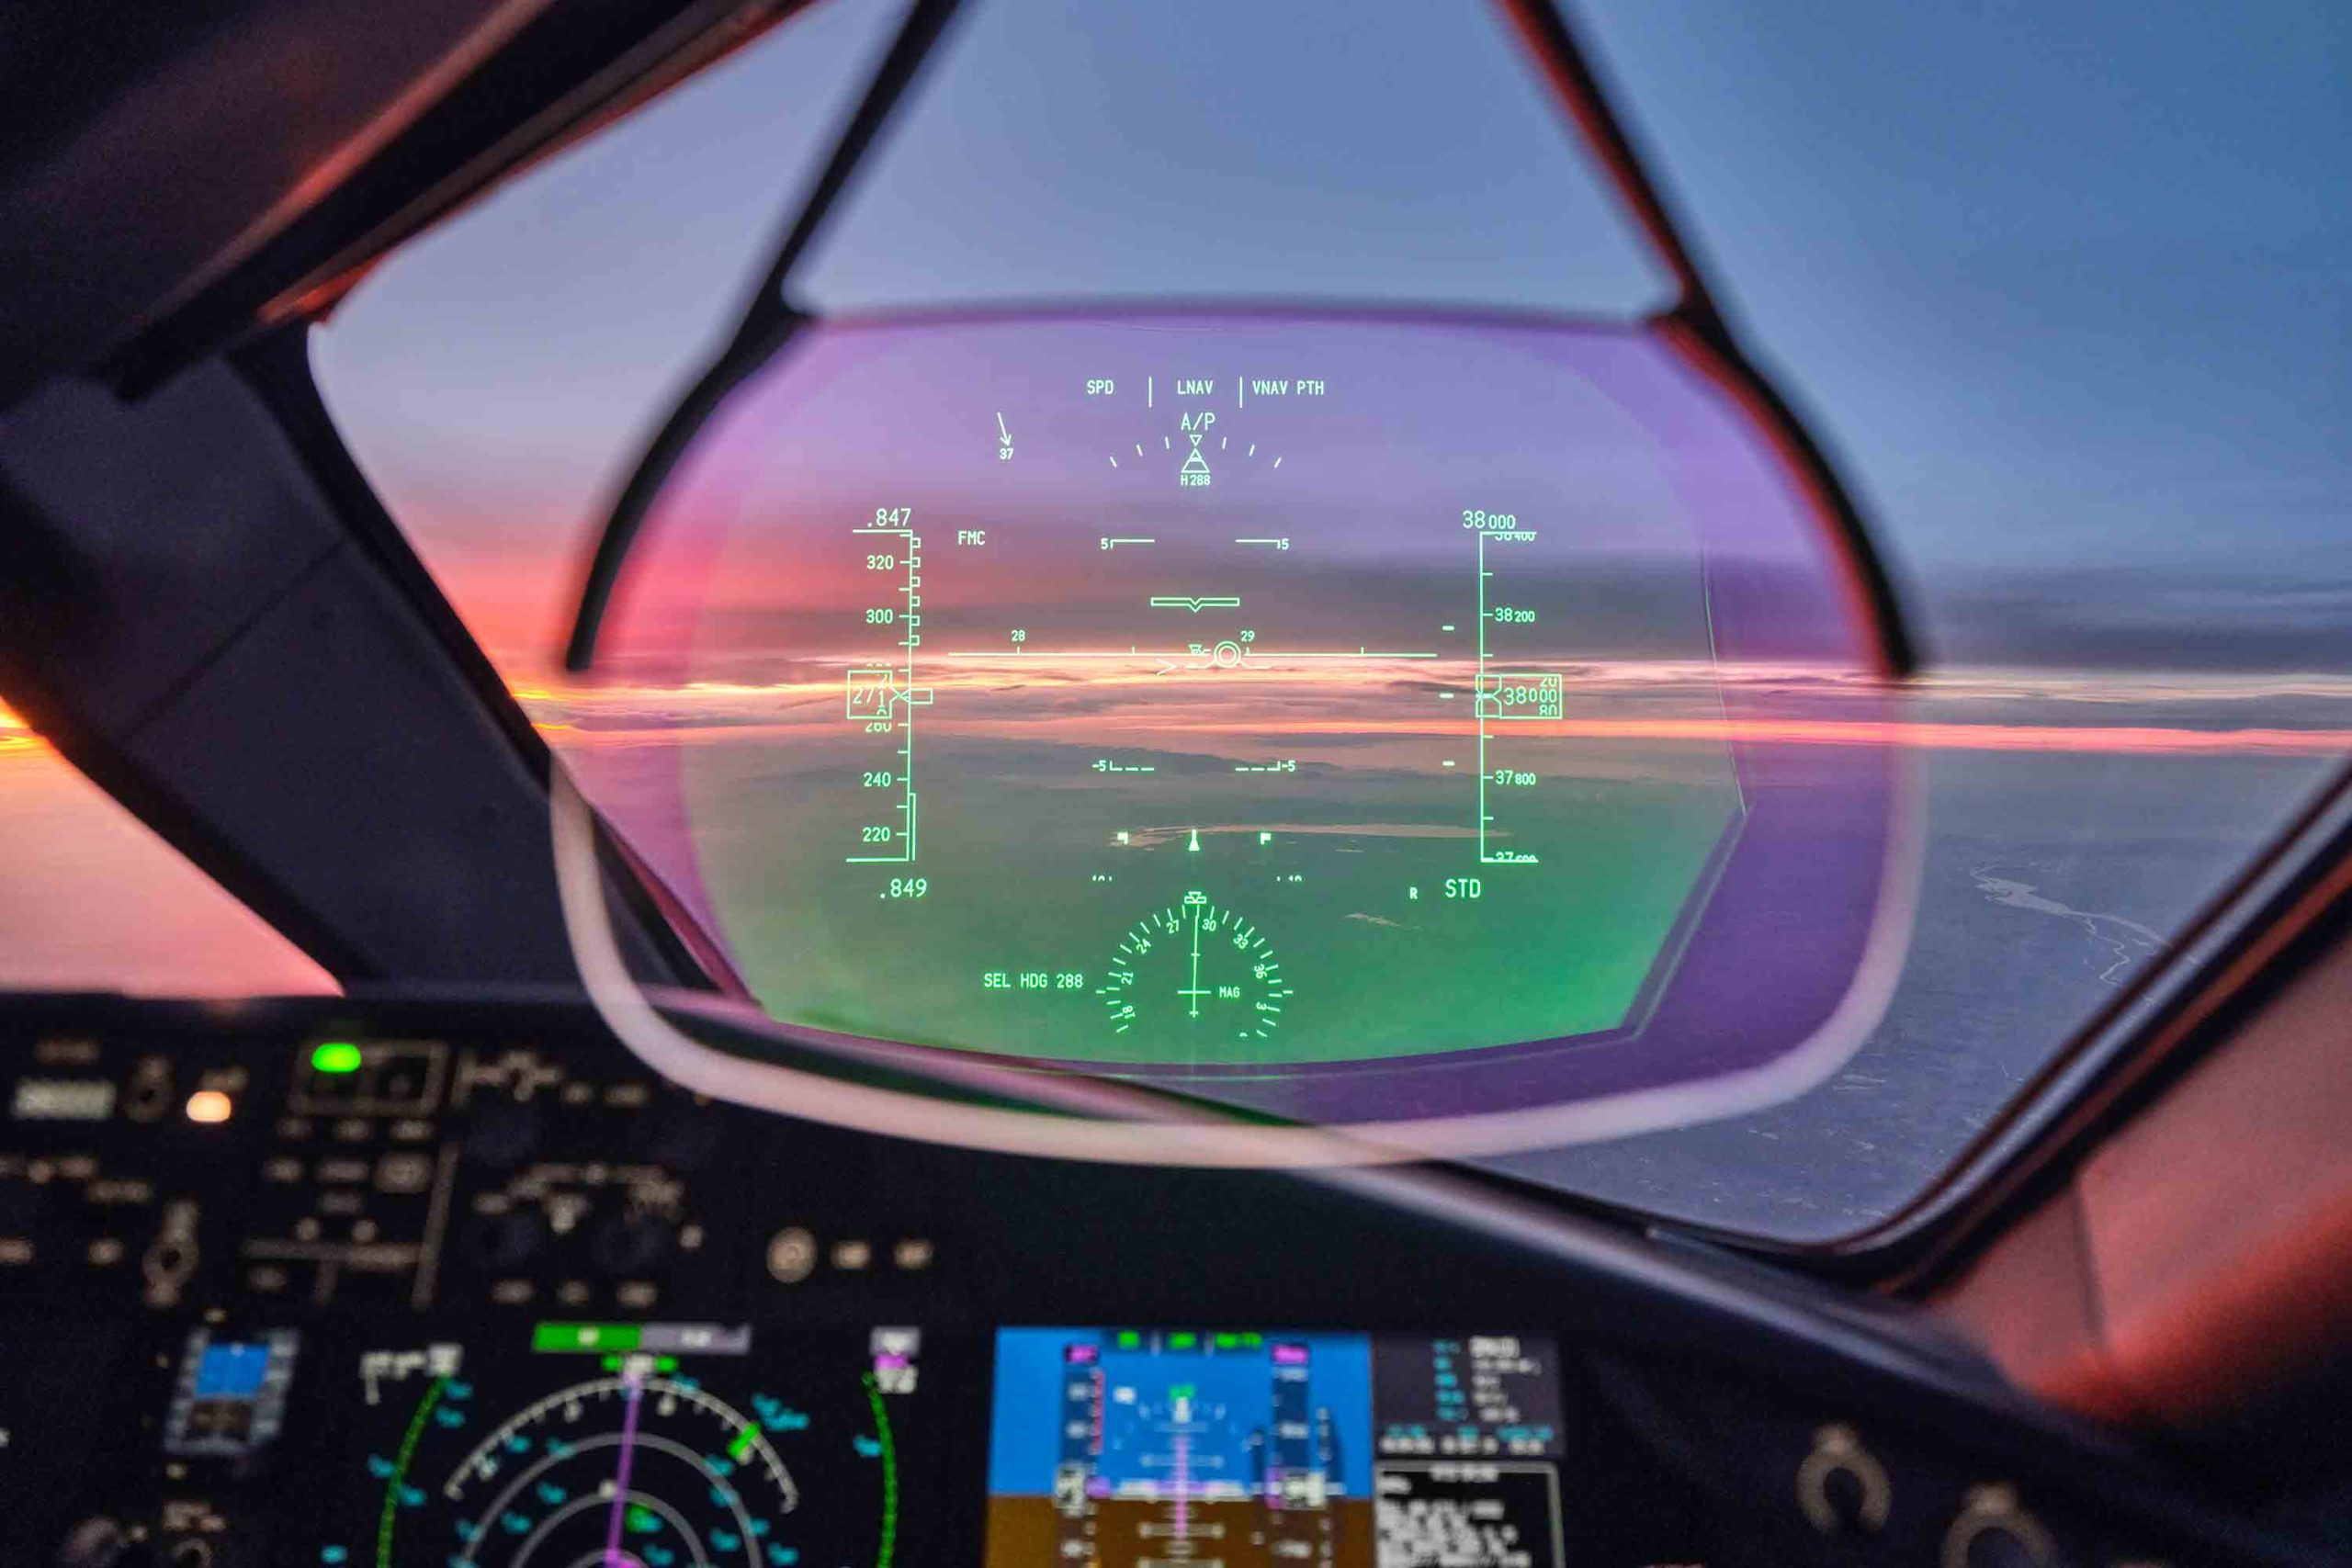
\includegraphics[scale=0.12]{obrazky-figures/787HUD.jpg}
\caption{HUD Boeing 787 Dreamliner\texttrademark{}. Prevzaté z~\cite{fotoB787}.}{\label{787hud}}
\end{figure}
    \item Digitálne head-up displeje. Tento typ displeja nahradil dlho pretrvávajúci CRT displej. Napríklad americké letectvo prijalo plne digitálne HUD pre svoje modely F-22 Raptor až v~roku 2020.
    \item Systém syntetického videnia. Jedná sa o~systém, ktorý je kombináciou tradičného HUD obsahujúci funkcie vylepšeného a syntetického videnia. Tieto systémy zahŕňajú informácie získané z~rôznych senzorov, ktoré letún obsahuje. Sú to napríklad infračervené kamery. Vojenský piloti majú možnosť si aktivovať nočné videnie pomocou systému nočného videnia (FLIR). Nočné videnie je znázornené na obrázku \ref{nightHUD}.
    \begin{figure}[ht]
\centering
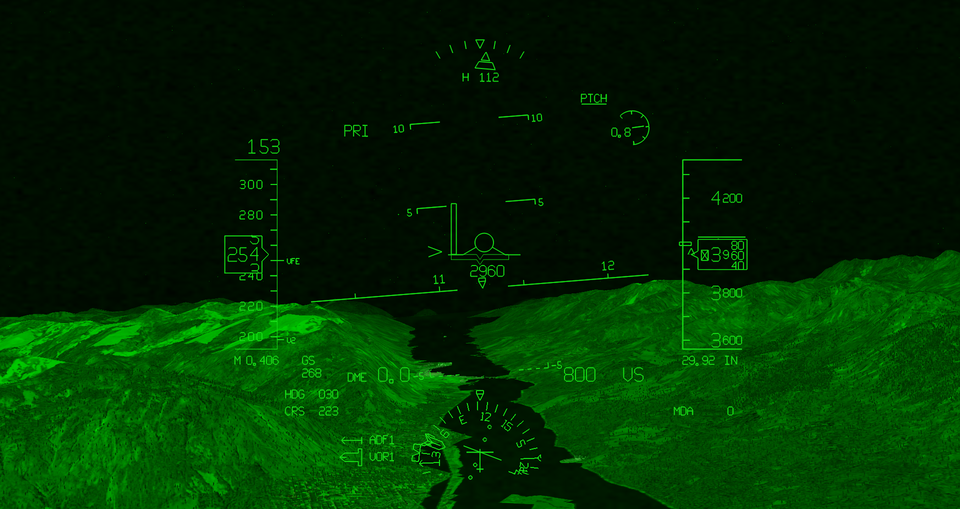
\includegraphics[height=8cm, width=13cm]{obrazky-figures/HUDs.png}
\caption{HUD so syntetickým videním. Prevzaté z~\cite{fotoSv2}.}{\label{nightHUD}}
\end{figure}
\end{itemize}

\subsection{Symbolika priehľadového displeja}
Cieľom symboliky pre HUD je  dodať nevyhnutné letové údaje a informácie potrebné pre~bezpečnú a efektívnu kontrolu letúna. Popis označenej symboliky, ktorá je na obrázku \ref{symbolika}:

\begin{enumerate}
    \item Vodoryska – symbol, ktorý predstavuje pozdĺžnu os letúna. Používa sa na určenie, či je letún v~udržovanom lete alebo nie.
    \item Rýchlosť – číslo, ktoré určuje indikovanú rýchlosť letúna. Nachádza sa v~rámčeku na~ľavej strane HUD.
    \item Horizont – čím vyššie sa letún nachádza, tým vyššie nad vizuálnym horizontom sa čiara objaví. Keď je značka smeru letu nad čiarou znamená to, že letún stúpa, v~opačnom prípade, že letún klesá. 
    \item Ľavý dátový blok – blok, ktorý obsahuje viacero údajov, ako sú uhol nábehu, Machovo číslo, násobok zaťaženia, indikácia času (TOD).
    \item Ukazovateľ náklonu – stupnica náklonu až do 90$^\circ$ doľava alebo doprava. Nachádza sa v~spodnej časti HUD.
    \item Stupnica sklonu – stupnica, ktorá udáva aktuálny sklon letúna vzhľadom k~horizontu.
    \item Pravý dátový blok – blok, ktorý obsahuje navigačné údaje pre pilota, ako sú napríklad informácie týkajúce sa systému automatického riadenia letu.
    \item Značka dráhy letu (FPM) – symbol v~tvare kruhu s~tromi čiarami, ktorý predstavuje bod, ku ktorému letún letí. Používa sa hlavne pri pristávaní a ďalších manévroch. 
    \item Nadmorská výška letúna (ALT) – číslo, ktoré reprezentuje aktuálnu nadmorskú výšku letúna. Nadmorská výška môže byť barometrická alebo radarová. Nachádza sa v~rámčeku na pravej strane HUD.
    \item Stupnica kurzu – pohyblivá stupnica, ktorá zobrazuje kurz, na ktorý je letún nasmerovaný. Kurz nemusí byť smer, na ktorý letún skutočne letí. Rozdiel medzi kurzom a~smerom môže byť spôsobený na základe poveternostných podmienok.
\end{enumerate}

\begin{figure}[ht]
\centering
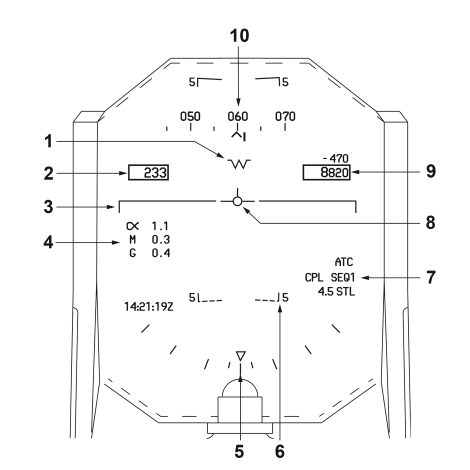
\includegraphics[height=8cm, width=8cm]{obrazky-figures/symbolikaHUD.png}
\caption{Symbolika HUD. Prevzaté z~\cite{fotoCS}.}{\label{symbolika}}
\end{figure}

\section{Helmet Mounted Display}
Prilbové displeje (HMD) nie sú v~súčasnosti až tak rozšírené. Najväčšie zastúpenie majú vo vojenskom priemysle. Nachádzajú sa na palubách letúnov štvrtej a taktiež aj piatej generácie \cite{HMDhelmet}.

\subsection{Popis prilbového displeja}
HMD je video projektor, ktorý získava rôzne informácie zo senzorov a zobrazuje ich na~vnútornej strane pilotovej prilby. Táto technológia umožňuje pilotom vnímať okolie, prekryté informáciami a na základe nich podniknúť potrebné kroky. HMD posielajú informácie priamo do výhľadu pilota bez ohľadu na to, kam otočia hlavu. Moderné HMD v~stíhacich letúnoch plnia viacero funkcií. Medzi tieto funkcie patrí napríklad zvýšenie celkového situačného podvedomia pilota, zlepšenie schopnosti držať oči mimo kokpitu letúna a taktiež dať pilotovi možnosť zamerať zbrane iba pohľadom na daný objekt alebo miesto. Táto možnosť patrí medzi najdôležitejšie. Práve takého HMD sa používajú na stíhacích letúnoch F-35~\cite{F35}, kde~sa pilot môže pozerať skrz letún akýmkoľvek smerom. Táto prilba \ref{HMD} je tak sofistikovaná a pôsobivá, že piloti F-35 lietajú pomocou dvoch displejov. Jeden sa nachádza v~kokpite a druhý na prilbe pilota. Je to jediný HMD na svete, ktorý je certifikovaný na to, aby~slúžil, ako primárny displej pilota. Schopnosť vidieť do všetkých smerov a mať informácie prezentované priamo vo zornom poli pilota je obrovská výhoda. Podľa štúdie Izraelského výskumného inštitútu sa počet bojových letúnov vylepšených o~HMD zvýšil trojnásobne~\cite{HMDhelmet}.

\begin{figure}[ht]
\centering
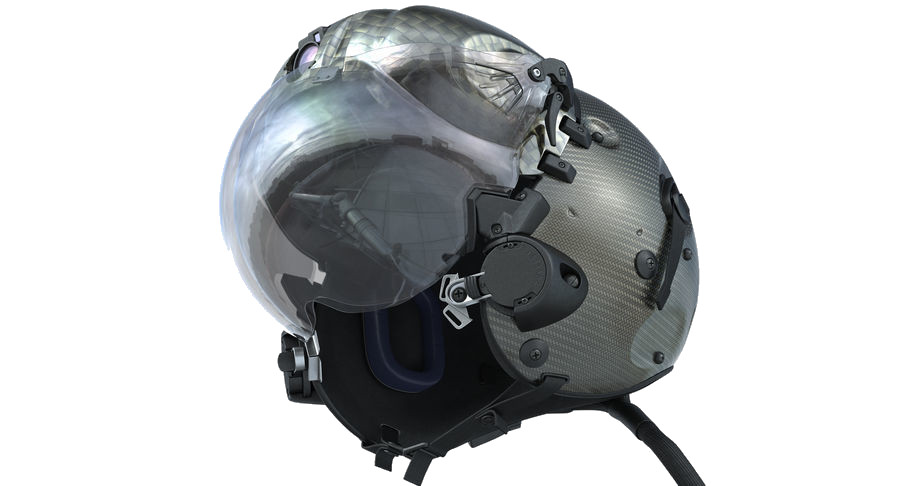
\includegraphics[scale=0.35]{obrazky-figures/HMDf35w.jpg}
\caption{Prilba pilota stíhacieho letúna F-35 obsahujúca HMD. Prevzaté z~\cite{fotoHelmet}.}{\label{HMD}}
\end{figure}

\subsection{Výhody prilbového displeja}
HMD patrí medzi najmodernejšie a najviac nápomocné systémy v~súčasnosti. Kľúčové výhody sú \cite{HMD}:

\begin{itemize}
    \item poskytuje dobré situačné povedomie,
    \item integrovaný virtuálny HUD na priezore prilby obsahujúci informácie o~lete,
    \item možnosť nočného videnia, ktorá je zabudovaná do prilby,
    \item ľahká prilba s~optimálnym ťažiskom pre komfort pilota.
\end{itemize}

\subsection{Nevýhody prilbového displeja}
Okrem spomenutých výhod je potreba zvážiť aj niekoľko nevýhod \cite{HMDnevyhody}:

\begin{itemize}
    \item Ak je hustota prezentovaných informácií príliš vysoká, môže sa zhoršiť viditeľnosť vonkajšieho sveta.
    \item Príliš veľké množstvo informácií na HMD môže pritiahnúť pozornosť pilota natoľko, že stratí pozornosť n vonkajší svet.
    \item Znížená priehľadnosť zrkadla HMD môže ovplyvniť pohľad a znížíť vnímanie farieb.
    \item Pri dlhom používaní môže dôjsť k~únave očí alebo bolesti hlavy.
\end{itemize}

Niekoľko z~týchto škodlivých faktorov bolo zistených empirickými výskumami. Rash et al hlásil poruchy zraku u~pilotov helikoptér, pri používaní systému, ktorý umožňuje lety v~noci a za zlého počasia. V~dotazníku až 92\% pilotov uviedlo zrakové problémy ako zrakové nepohodlie, dvojité videnie, dezorientáciu či bolesť hlavy počas letu a taktiež po~ňom. Howarth a Costello zistili príznaky kinetózy práve, keď boli použité biokulárne HMD. Dôvodom môže byť zmyslový konflikt, keď pohyby hlavy sú vnímané vestibulárnym ale nie zrakovým systémom \cite{HMDnevyhody}.

%----------------------------NAVRH-----------------------------------
\chapter{Návrh vizualizácie letových dát v~prostredí letového displeja}
Vytvorenie dobrého návrhu je veľmi dôležité. Pri nesprávnom návrhu môže táto pomôcka skôr uškodiť, ako pomôcť. Pri vytváraní návrhu sa autor snažil získať podrobnejšie informácie ohľadom prístrojov letúna a identifikovať, aké prístroje sú najviac využívané počas letu. Po získaní týchto informácií bolo pristúpené k~vytváraniu návrhu HUD. Pri začiatku vytvárania návrhu bolo dôležité dodržanie štruktúry systému.

\section{Štruktúra systému}
Počítač HUD získava informácie zo zdrojov, medzi ktoré patria Air Data Computer (ADC), inerčný referenčný systém (IRS), rádionavigačné prístroje, rádiovýškomer, gyroskopické prístroje. Tieto informácie prepočítava do súradnicovej osi x a osi y a následne ich dodáva generátoru symbolov na spracovanie grafického výstupu. Vďaka týmto údajom vytvorí generátor symbolov nevyhnutné súradnice pre symboli, ktoré odošle zobrazovaciemu zariadeniu. Tieto údaje sú následne duplikované a odoslané do počítačov. Prvý súbor je odoslaný do HUD počítača a ten druhý do paralelného počítača. Paralelný počítač posiela údaje do~kontrolnej jednotky. Táto jednotka získava dva súbory údajov, a to jeden z~HUD počítača a druhý z~paralelného počítača. Medzi týmito súbormi nemôže nastať odchýlka. V~prípade, že nastane, zašle zobrazovacej jednotke chybovú hlášku. 

Na obrázku \ref{oblasti} je znázornené rozdelenie oblastí, v~ktorých sa zobrazujú rozličné získané údaje. Popis označenej symboliky:

\begin{figure}[h]
 \begin{minipage}{.48\textwidth}
 \centering
  \begin{enumerate}
    \item oblasť kurzu,
    \item oblasť výšky,
    \item hlavná oblasť,
    \item pravý priestor údajov,
    \item oblasť stupnice náklonu a údajov,
    \item ľavý priestor údajov,
    \item oblasť rýchlosti.
\end{enumerate}
  \end{minipage}%
  \hfill
  \begin{minipage}{.48\textwidth}
  \centering
  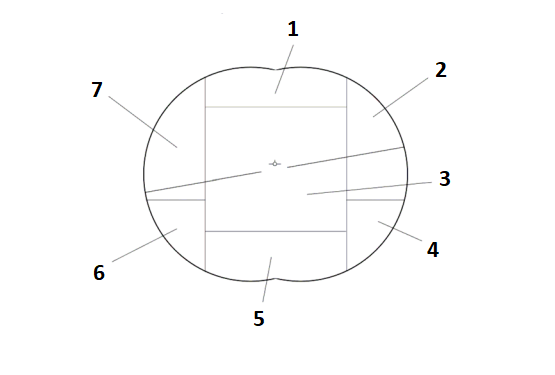
\includegraphics[scale=0.41]{obrazky-figures/oblastiHUD.png}
  \caption{Rozloženie oblastí na priehľadovom displeji. Prevzaté z~\cite{HUDkniha}.}{\label{oblasti}}
  \end{minipage}% 
\end{figure}
\newpage

\section{Vlastný návrh}
Hlavné zameranie pre vytvorenie návrhu je vytvoriť vizualizáciu dát tak, aby bola pre užívateľa jednoduchá a obsahovala všetky potrebné prvky, ktoré bude potrebovať. Návrh je zameraný a vytvorený pre letún typu eVTOL podporujúci virtuálnu realitu. Tento typ letúna môžete vidieť na obrázku \ref{evtol}. Na týchto obrázkoch sú zobrazené obe možné varianty pozície vrtúl. Zatiaľ čo na ľavom obrázku sú nastavené pre horizontálny let letúna, tak na~pravom obrázku sú propulzory nastavené na vertikálny vzlet. Návrh je vytvorený na základe získaných informácií o~HMD, ktorý patrí medzi najmodernejšie systémy v~súčasnosti. Pri vytváraní návrhu som sa zameral hlavne na prístoje letúna, ktoré su najdôležitejšie pri vykonávaní letu. Medzi najužitočnejší a najpotrebnejší indikator patrí umelý horizont, ktorý je znázornený na obrázku \ref{poloha}. Vďaka tomuto indikátoru sme schopný riadiť letún a~informovať sa o~jeho správaní.

\begin{figure}[ht]
\centering
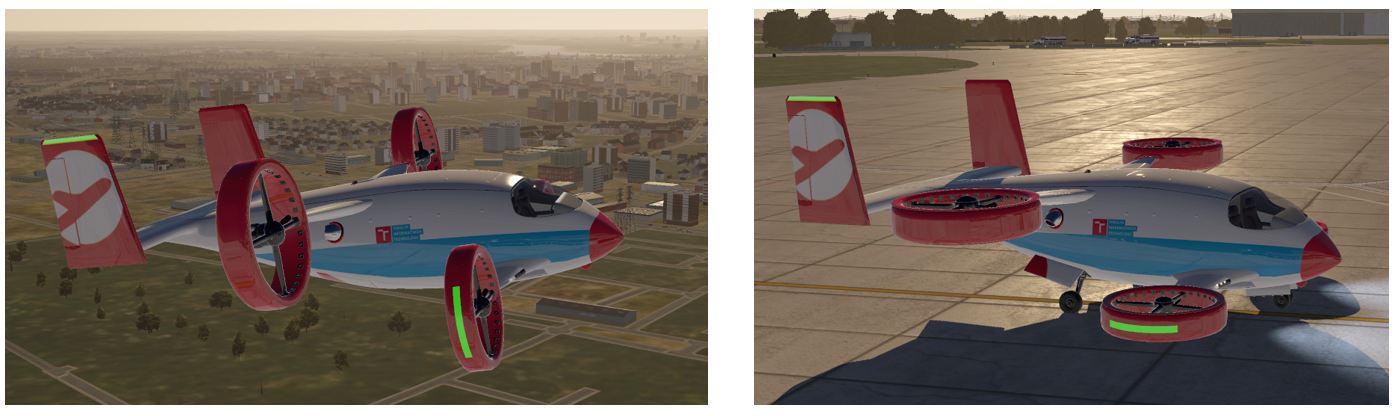
\includegraphics[scale=0.4]{obrazky-figures/eVTOL_aircraft.png}
\caption{Model letúna AG-4 eVTOL v2.0.}{\label{evtol}}
\end{figure}

Na obrázku \ref{vlastny_navrh} je znázornený prvý navrhnutý HUD. Pri vytvárani tohoto návrhu som sa z~časti išpiroval displejom, ktorý sa nachádza v~stíhacích letúnoch F-35. Po skonzultovaní a naštudovaní viacerých článkov, dospel autor k~záveru, že návrh ide správnym smerov ale taktiež je potreba upraviť umiestnenie jednotlivých častí HUD alebo pridanie informácií, ktoré by mohli byť nápomocné pri vykonávaní vertikálnych manévrov pri vzlete alebo pristáti. Tento návrh obsahuje časti medzi ktoré patrí stupnica smeru (kurzu), značka smeru letu, stupnica klopenia, čiara horizontu, ukazovateľ aktuálnej výšky a rýchlosti letúna a~indikátor klonenia.
\newpage
\begin{figure}[ht]
\centering
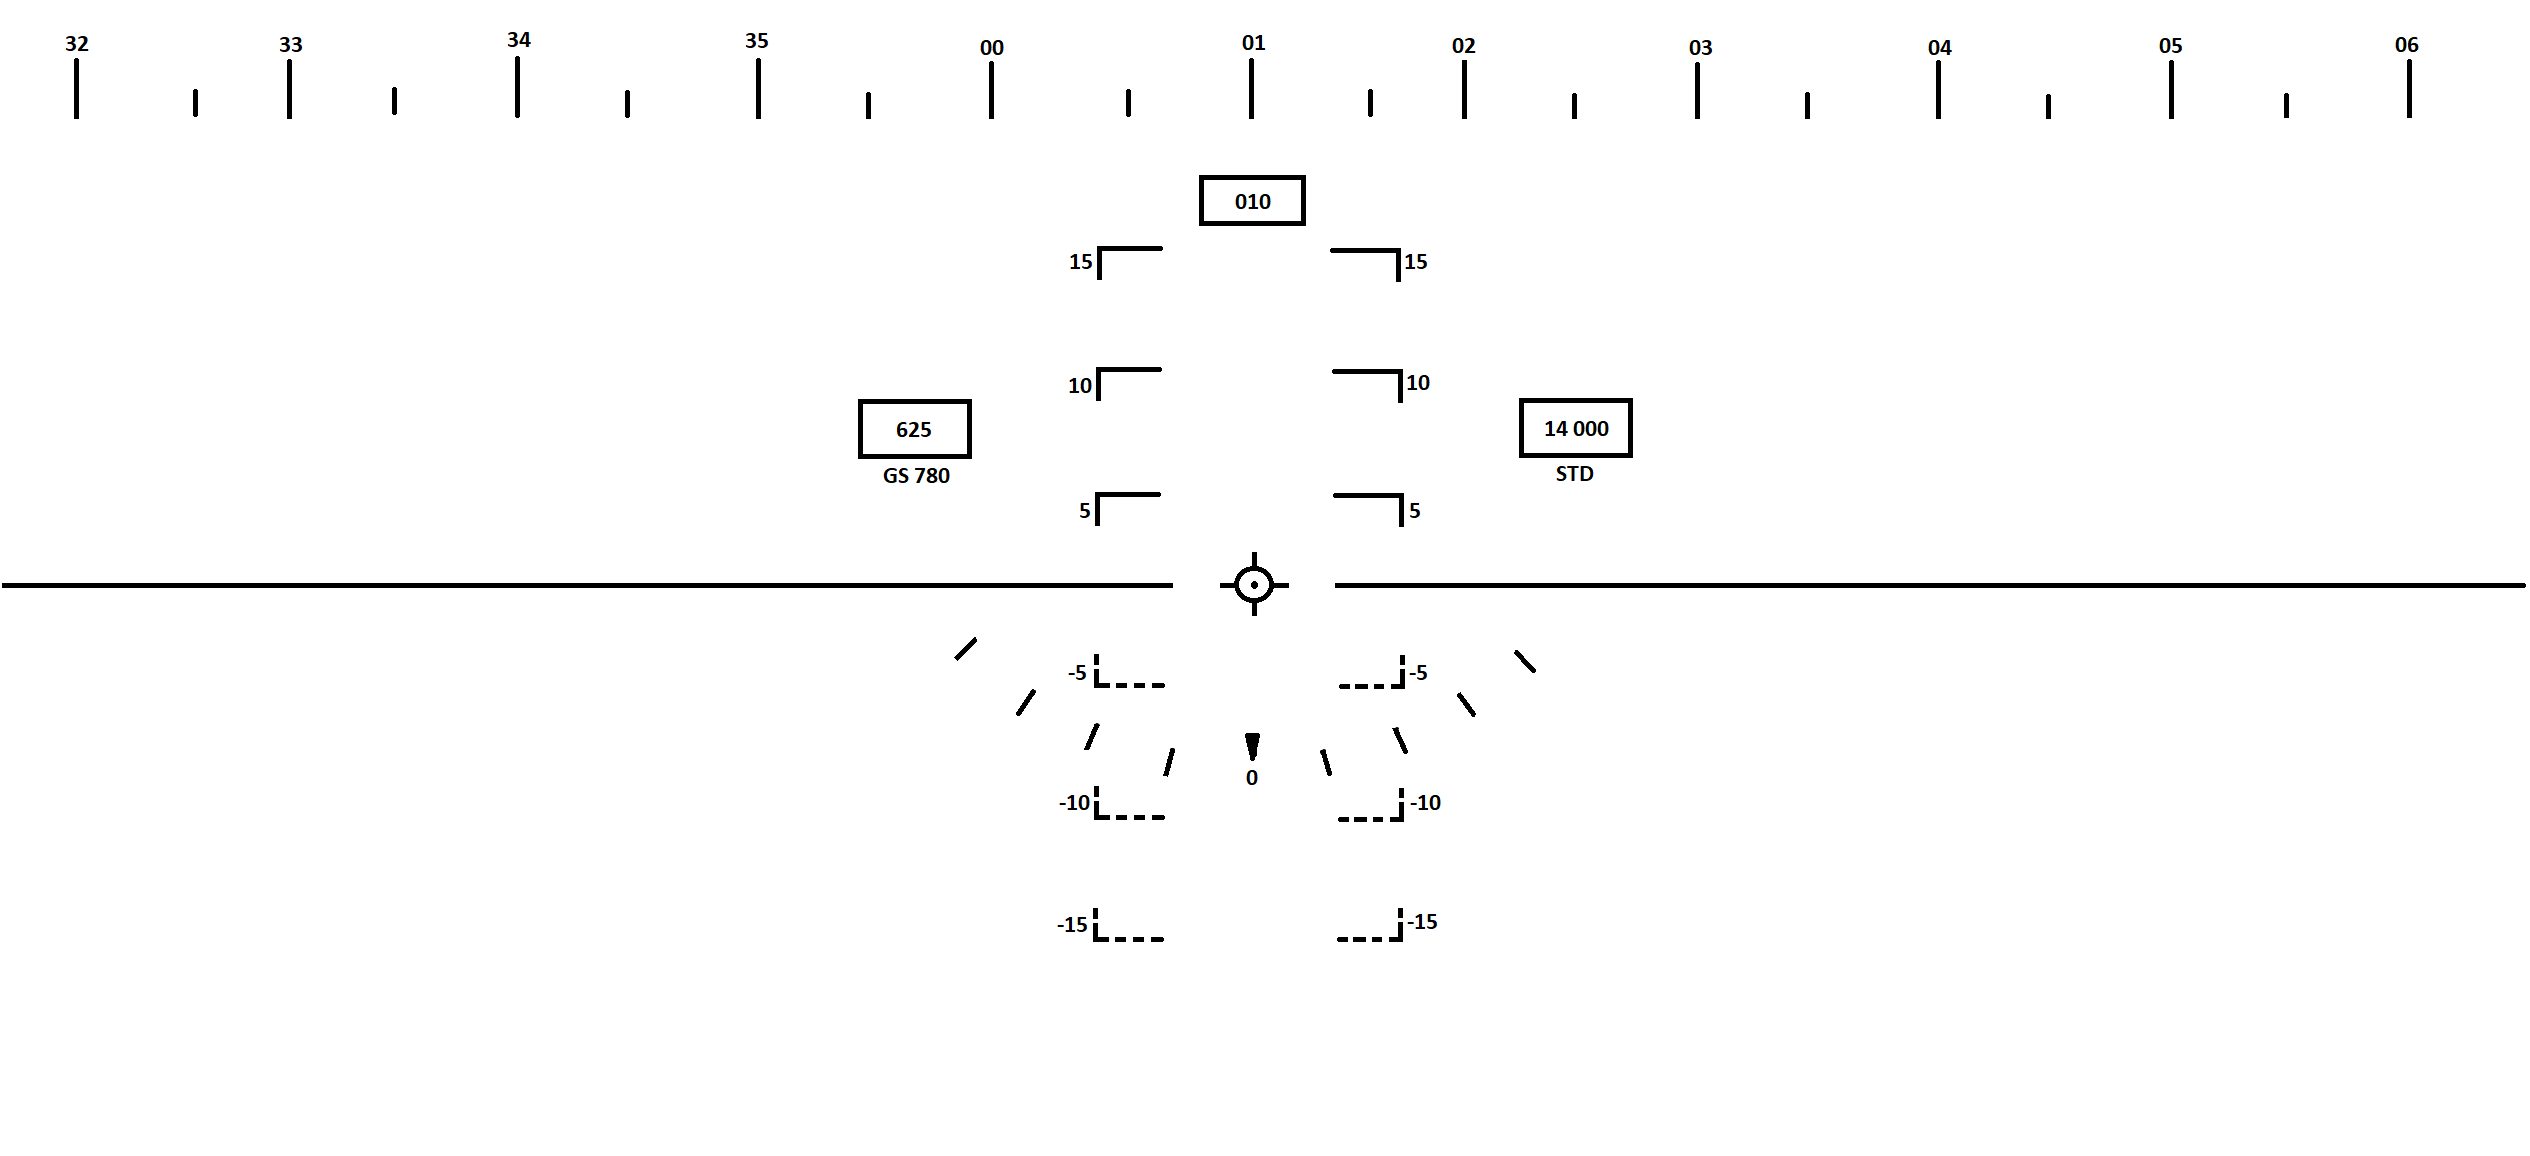
\includegraphics[height=7cm, width=14cm]{obrazky-figures/HUD_navrh2.png}
\caption{Prvý návrh HUD.}{\label{vlastny_navrh}}
\end{figure}

Na obrázku \ref{secondHUD} je znázornený upravený návrh HUD. Displej sa líši od prvého tým, že na ľavej strane je zobrazený datový blok, ktorý obsahuje tri hodnoty a to sú uhol nábehu, Machovo číslo a násobok zaťaženia. V~tejto časti môže byť taktiež zobrazená indikácia času, značená skratkou (TOD). Na pravej strane je znázornený indikátor klolenia, ktorý je presunutý zo stredovej časti oproti pôvodnemu riešeniu HUD. Posledná zmena nastala v~ukazovateli rýchlosti, ktorý je upravený pre prehľadnejšie ukazovanie výšky, ktorá sa môže rýchlo meniť. Tento návrh bol kvalitnejší oproti pôvodnému avšak nebol úplne prehľadný.

\begin{figure}[ht]
\centering
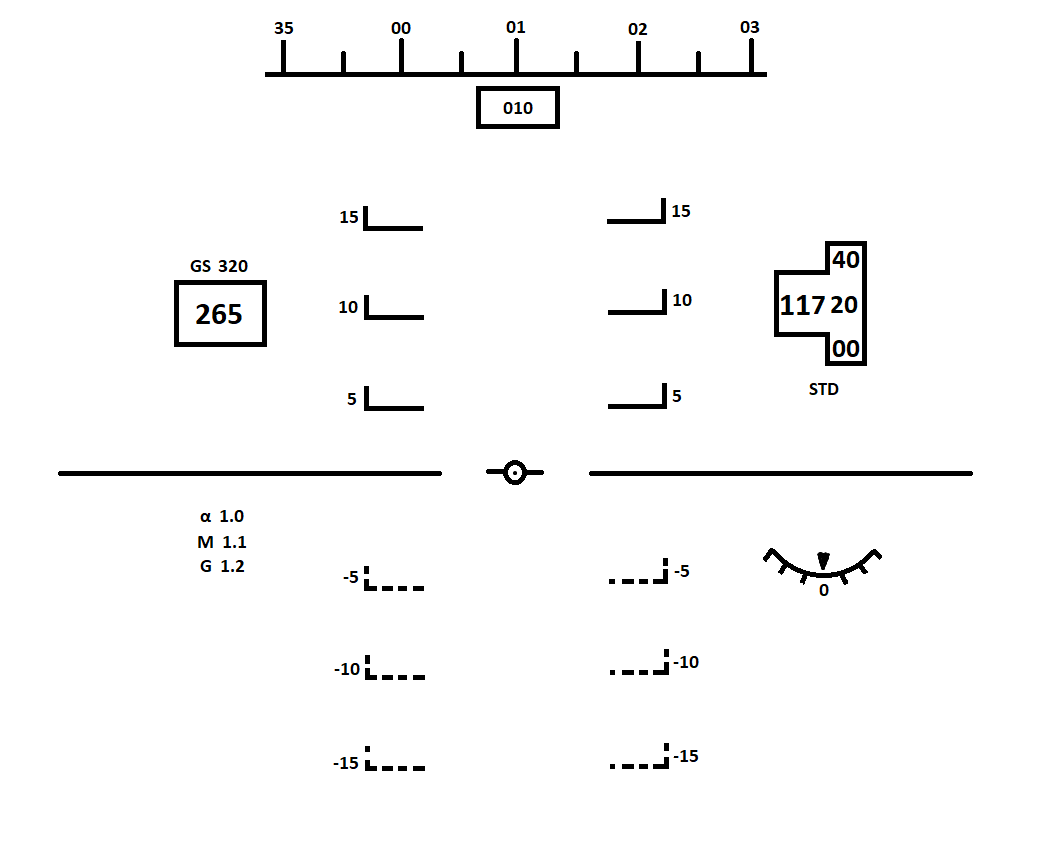
\includegraphics[scale=0.35]{obrazky-figures/secondHUD.png}
\caption{Druhý návrh HUD.}{\label{secondHUD}}
\end{figure}
\newpage

Na základe toho, vznikol tretí návrh, ktorý obsahuje viaceré zmeny. Tento návrh, ktorého základ je zobrazený na obrázku \ref{finalHUD} je založený na základe spomínaného umelého horizontu letúna.
Hlavné časti finálneho návrhu sú:
\begin{itemize}
    \item Stupnica smeru (kurzu) - táto stupnica sa nachádza na samom vrchu HUD. Označuje kurz, na ktorý je letún nasmerovaný. Pod touto stupnicou sa nachádza rámček, v~ktorou je znázornený aktuálny kurz letúna. Tým, že návrh je realizovaný v~3D priestore pomocou virtuálnej reality, tak táto stupnica kurzu je zobrazená ako 3D. Céla stupnica je zaoblená do polkruhu. Vďaka tomuto zaobleniu, to dodáva väčšiu prehľadnosť. Toto zaoblenie môžete vidieť na obrázku \ref{3Dkurz}.
    \begin{figure}[ht]
\centering
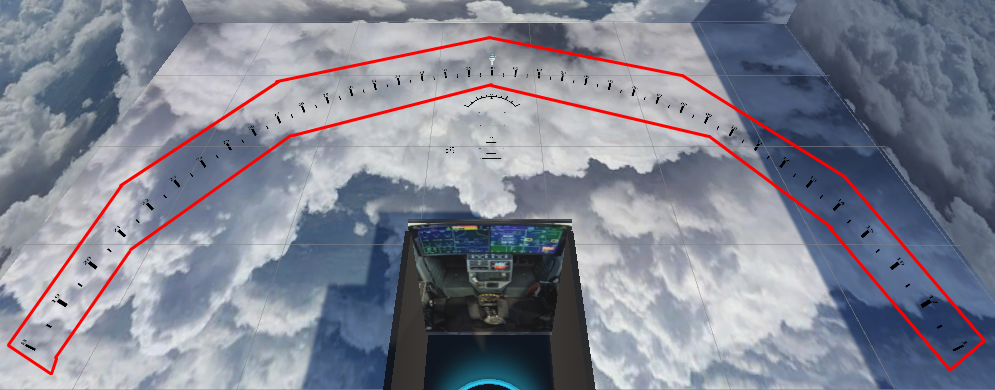
\includegraphics[scale=0.4]{obrazky-figures/3Dkurz.png}
\caption{Zaoblená stupnica smeru (kurzu).}{\label{3Dkurz}}
\end{figure}
    \item Stupnica klopenia - nachádza sa v~strednej časti HUD a predstavuje pozdĺžny sklon, pod akým letún letí. Toto označenie sa značí po 5$^\circ$ až po sklon 60$^\circ$. Avšak od hodnoty 50$^\circ$ začínajú červené varovné šípky, ktoré slúžia na informovanie o~nebezpečnom sklone. Toto označenie je znázornené na obrázku \ref{warning}.
    \begin{figure}[ht]
\centering
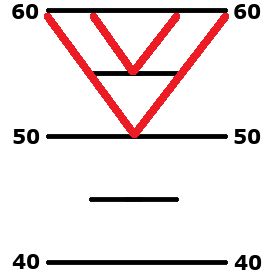
\includegraphics[scale=0.61]{obrazky-figures/warning.png}
\caption{Varovné označenie pri dosiahnutí nebezpečného sklonu.}{\label{warning}}
\end{figure}
    \item QNH - tlak nastavený tak, aby prístroj ukazoval jeho výšku nad hladinou mora. Štandardné nastavenie tlaku sa označuje skratkou STD, ktoré reprezentuje hodnotu 1013 hPa.
    \item Čiara horizontu - nachádza sa po bokoch značky smeru letu a predstavuje horizont. Na základe týchto dvoch vecí sme schopný určiť, v~akom štádiu sa letún nachádza. 
    \item Aktuálna rýchlosť - nachádza sa v~rámčeku na ľavej strednej časti HUD. Toto číslo určuje aktuálnu vzdušnú rýchlosť letúna.
    \item Aktuálna rýchlosť voči zemi - nachádza sa v~rámčeku na ľavej strednej časti HUD nad aktuálnou rýchlosťou letúna. Toto číslo určuje aktuálnu rýchlosť letúna voči zemi. Táto rýchlosť sa značí skratkov (GS).
    \item Ťah motorov - tieto štyri hodnoty sa nachádzajú v~rámčekoch na ľavej strane pod~aktuálnou rýchlosťou letúna. Horné dve hodnoty informujú o~ťahu predných motorov. Spodné dve hodnoty znázorňujú ťah zadných motorov letúna. Rozloženie propulzorov na letúne je znázornené na obrázkoch \ref{prednyMotor} a \ref{zadnyMotor}.
    \item Aktuálna výška - nachádza sa v~rámčeku na pravej strednej časti HUD. Toto číslo značí aktuálnu nadmorskú výšku letúna.
    \item Indikátor klonenia - tento indikátor sa nachádza na hornej časti pod stupnicou smeru (kurzu) a obsahuje päť výbežkov na každej strane, ktoré značia 10$^\circ$, 20$^\circ$, 30$^\circ$, 45$^\circ$ a~60$^\circ$ klonenie.
\end{itemize}
\begin{figure}[ht]
\centering
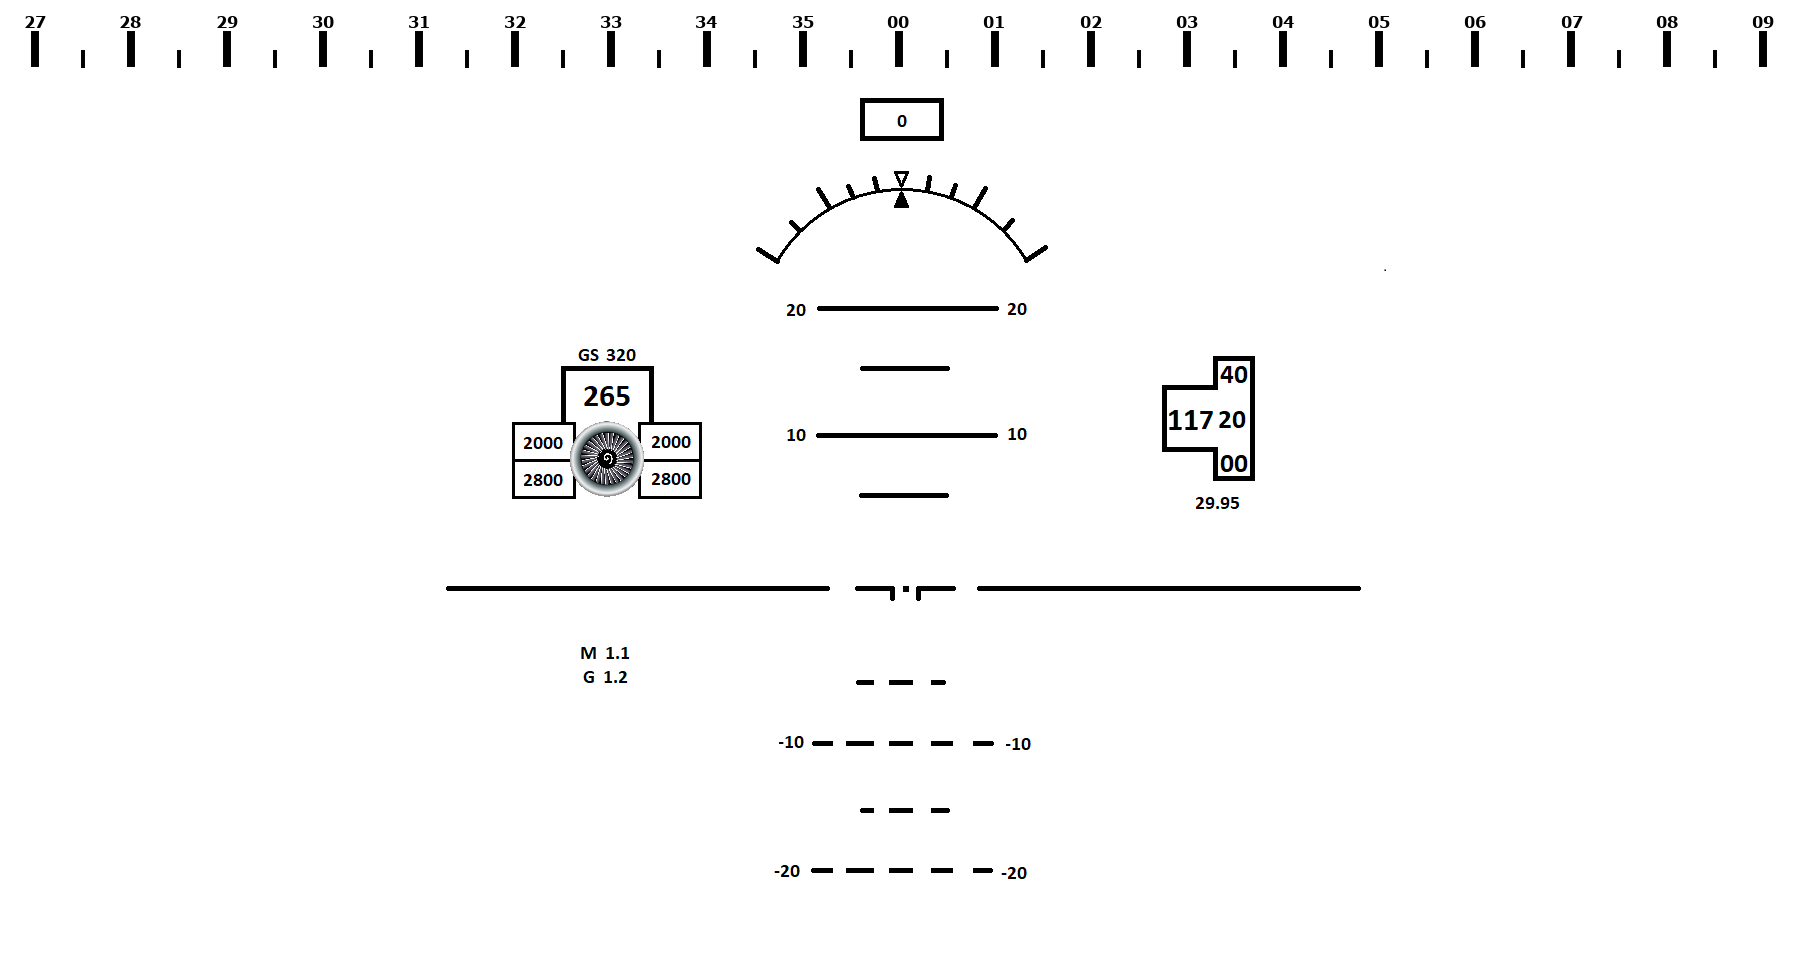
\includegraphics[scale=0.3]{obrazky-figures/finalHUDf.png}
\caption{Tretí návrh HUD.}{\label{finalHUD}}
\end{figure}

\begin{figure}[h]
 \begin{minipage}{.48\textwidth}
  \centering
  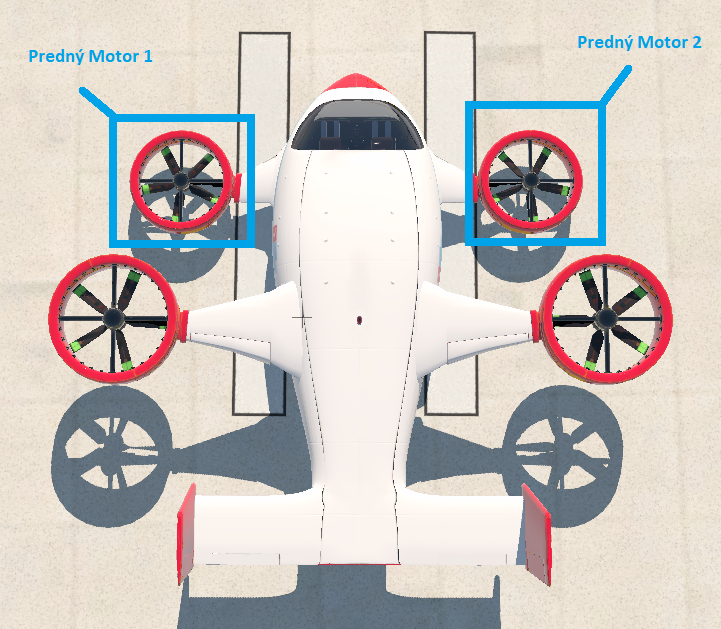
\includegraphics[scale=0.32]{obrazky-figures/motoryP.png}
  \caption{Predné propulzory letúna eVTOL.}\label{prednyMotor}
  \end{minipage}%
  \hfill
  \begin{minipage}{.48\textwidth}
  \centering
  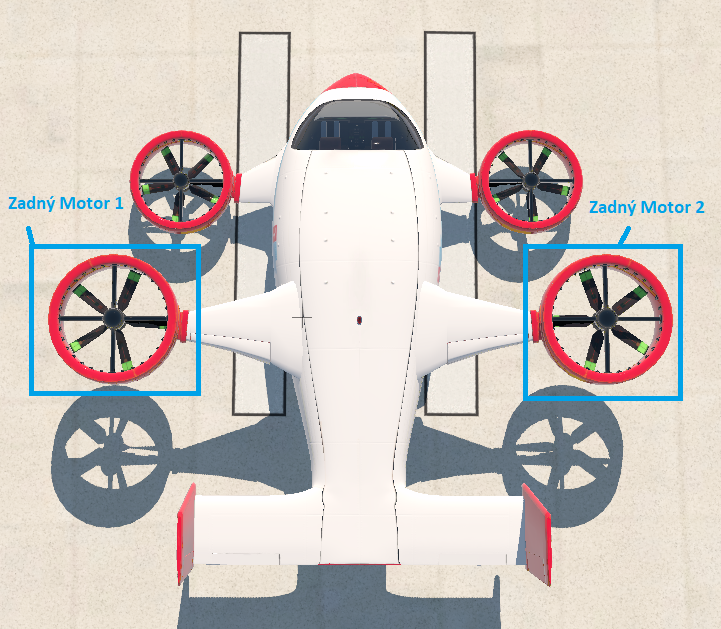
\includegraphics[scale=0.32]{obrazky-figures/motoryZ.png}
  \caption{Zadné propulzory letúna eVTOL.}\label{zadnyMotor}
  \end{minipage}% 
\end{figure}
\newpage

Tieto časti sú rozdelené do 2 typov displejov. Jeden displej je pevný, čo znamená, že je klasicky umiestnený na pevnom mieste v~zornom poli pilota. Tento typ HUD obsahuje riadiace informácie o~letúne ako sú stupnica smeru, indikátor klonenia. Nad stupnicou smeru (kurzu) sa nachádza ikonka v~tvare riadiacej veže letovej prevádzky, ktorá naznačuje, na~akom kurze sa nachádza zadané letisko. Ikonka veže je znázornená na obrázku \ref{tower}. Táto vežička sa taktiež pohybuje v~rovnakej línii ako zaoblená stupnica kurzu. Druhá časť HUD sa pohybuje s~hlavov pilota. Toto slúži hlavne pre získanie prehľadu o~lete počas rôznych manévrom, kedy sa pilot nemusí pozerať len rovno pred seba ale môže sa pozerať aj do bokov. V~tejto časti sú zobrazené výkonové informácie o~letúne. Medzi ne patrí aktuálna rýchlosť, aktuálna výška letúna, ťah motorov či kurz na ktorý letún aktuálne letí. Na obrázku \ref{rozdelenie} sú zakrúžkované časti HUD, ktoré sa pohybujú.

\begin{figure}[ht]
\centering
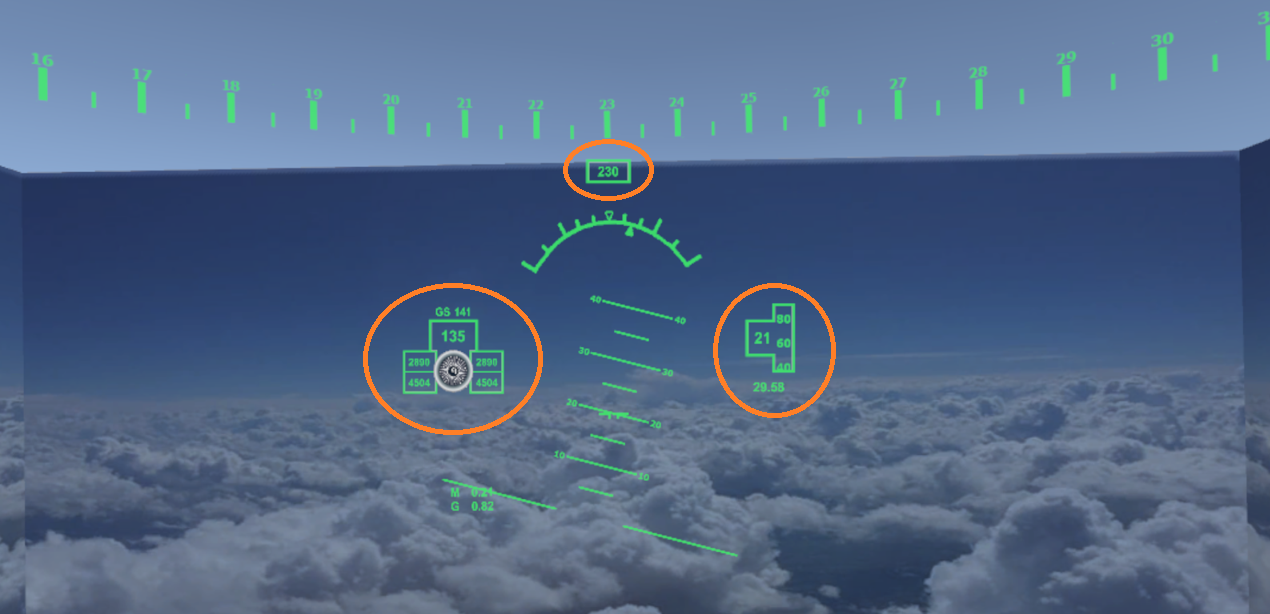
\includegraphics[scale=0.45]{obrazky-figures/rozdelenie.png}
\caption{Pohybujúce sa časti HUD.}{\label{rozdelenie}}
\end{figure}

\begin{figure}[ht]
\centering
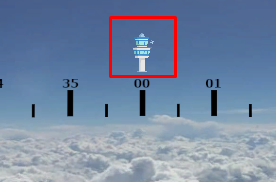
\includegraphics[]{obrazky-figures/Tower.png}
\caption{Ikona znázorňujúca navigačné údaje.}{\label{tower}}
\end{figure}

%-----------------------------IMPLEMENTACIA-----------------------------------
\chapter{Implementácia v~prostredí leteckého simulátora}
V~tejto kapitole je popísaný postup pri implementácií HUD. Taktiež sú tu popísané aplikácie, ktoré boli používané pri vytváraní priehľadového displeja.

\section{Popis implementácie}
Počas implemetácie boli použité viaceré applikácie. Pri vytváraní návrhu bola použitá aplikácia GIMP, ktorá slúžila na vytvorenie návrhu priehľadového displeja a rovnako na vytvorenie jednotlivých častí HUD a upravenie ich tak, aby boli čo najprehľadnejšie. Pre prácu s~týmito časťami bola použitá aplikácia Unity, ktorá podporuje virtuálnu realitu, takže bola veľmi vhodná pre túto prácu. V~tejto aplikácií bol používaný Unity Editor, kde bola vytvorená 3D scéna, do ktorej boli umiestnené jednotlivé časti HUD. Po správnom umiestnení jednotlivých prvkov následovalo naprogramovanie ich logiky. Na naprogramovanie logiky sa používal programovací jazyk \textit{C\#}, v~ktorom sa používala trieda \textit{MonoBehaviour}. Z~tejto triedy je odvodený každý skript Unity.

Správne fungovanie obrazových častí HUD ako je napríklad ukazovateľ výšky alebo stupnica smeru je spracované pomocou štruktúry \textit{Rect} v~UnityEngine. Jedná sa o~obdĺžnik definovaný polohou \textit{X} a \textit{Y}, šírkou a výškou. Unity používa množstvo 2D súradnicových priestorov, z~ktorých väčšina definuje \textit{X} ako rastúce doprava a \textit{Y} ako rastúce nahor. Obdĺžniky sú v~tomto prípade špecifikované súradnicami \textit{X} a \textit{Y} každej z~jeho hrán, ktoré sa nazývajú \textit{xMin, xMax, yMin a yMax}. Označenie súradníc je znázornené na obrázku \ref{rectangle}.

Pri častiach ako indikátor klonenia alebo ukazovateľ sklonu je funkčnosť implementovaná na základe otáčania objektov pomocou triedy Transform.Rotate. Rotáciu je možné zadať vo svetových osiach alebo v~lokálnych osiach.

Pre získavanie dát z~hry X-Plane 11 sa využíva plugin X-Plane Connect Toolbox. Pre~získanie dát je použitý programovací jazyk C v~ktorom sa volá viac krát funkcia \textit{getDREF(XPCSocket sock, const char* dref, float values[], int* size)}, ktorá vracia 0 v~prípade úspechu alebo záporné číslo v~prípade neúspechu. Prvý parameter reprezentuje soket, ktorý sa má použiť na odoslanie príkazu. Druhý parameter predstavuje názov dataref, ktorý chceme získať. Tretí parameter predstavuje pole, v~ktorom budú uložené hodnoty dataref. Dataref predstavuje databázu veľkého množstva rôznych typov dát, ktoré sme schopný získáť od hry X-Plane 11. Posledný parameter značí alokovanú veľkosť pola, v~ktorom je uložený výsledok. Pre získanie dát pitch a roll je použitá funkcia \textit{getPOSI(XPCSocket sock, float values[7], char ac)}. Vďaka tejto funkcií je možné získať viacere informácie týkajúce sa polohy letúna. Princip získavania hodnôt je podobný ako pri funkcií \textit{getDREF} avšak rozdiel je v~tom, že jedným volaním funkcie \textit{getPOSI} dokážeme získať až sedem hodnôt naraz. Tieto dáta sú vypísané do terminálu, kde sa kontrolujú ich hodnoty. Získavanie dát môžete vidieť na obrázku \ref{getData}. Po získaní požadovaných dát vďaka tejto funkcií, sú jednotlivé hodnoty ukladáné do samostatných textových súborov, z~ktorých sú následne extrahované a použité pri naprogramovaní funkcionality jednotlivých častí HUD v~aplikáci Unity. Pri~pohyblivých častiach HUD sa pracuje s~dátami, ktoré obsahujú viacero desatinných miest z~dôvodu, aby pohyby častí displeja boli čo najplynulejšie.
\begin{figure}[ht]
\centering
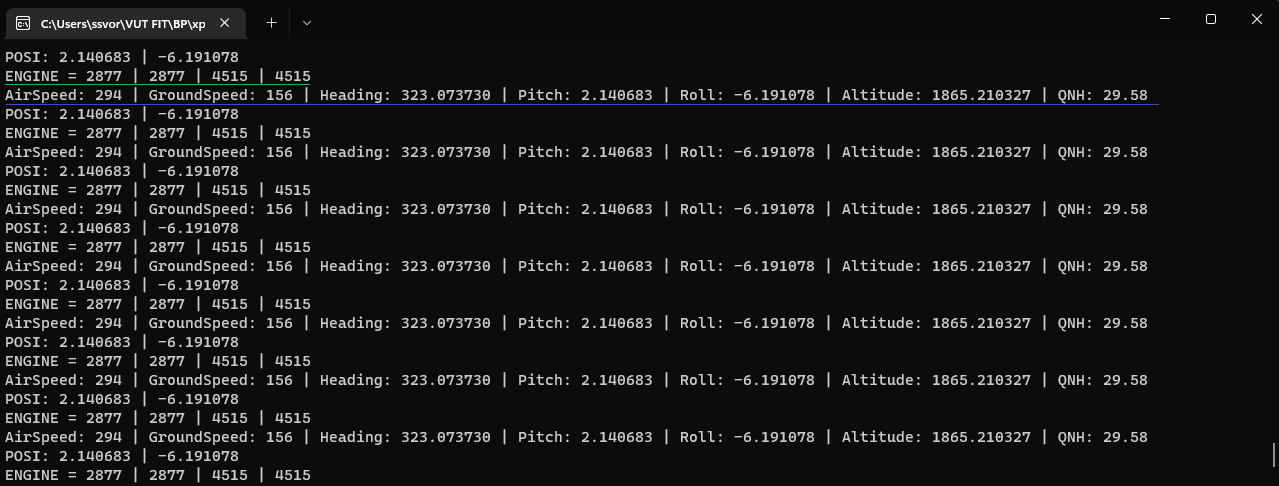
\includegraphics[width=15cm, height=8cm]{obrazky-figures/terminalData.png}
\caption{Vypisovanie získaných dát.}{\label{getData}}
\end{figure}

\begin{figure}[ht]
\centering
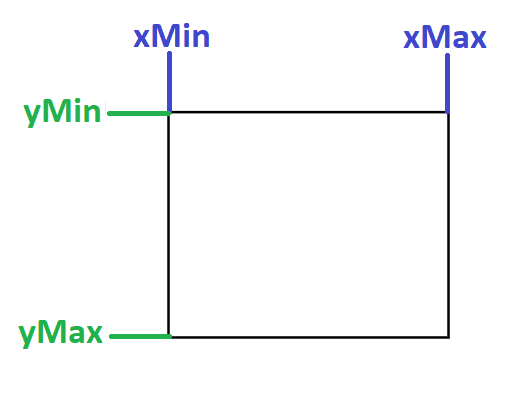
\includegraphics[scale=0.39]{obrazky-figures/rectangle.png}
\caption{Označenie súradníc X a Y.}{\label{rectangle}}
\end{figure}

\section{Použité nástroje}
Pri implementáci práce boli použité viaceré nástroje. Pre získavanie dát z~hry bol použitý X-Plane Connect Toolbox. Pre prácu s~jednotlivými časťami HUD bol použitý nástoj Gimp. Pre samostatný vývoj aplikácie bolo použité Unity, kde sa využívala virtuálna realita HTC Vive.

\subsection{X-Plane Connect Toolbox}
Jedná sa o~bezplatný, voľne dostupný nástroj pre Windows, Linux a macOS, ktorý umožňuje užívateľom prijímať v~reálnom čase informácie o~stave jedného alebo viacerých simulovaných vozidiel z~leteckého simulátora X-Plane 11 a ovládať vozidlá bežiace v~simulačnom prostredí X-Plane 11. Informácie je možné prijímať pomocou rôznych funkcií napísaných v~programovacích jazykoch \textit{C, C++, Java, MATLAB} alebo \textit{Python}. Súpravu nástrojov je možné použiť na zaznamenávanie údajov o~simulovaných letoch, vizualizáciu letových profilov, testovanie autopilotov a testovanie riadiacich algoritmov. Okrem toho, tento plugin umožňuje zobrazenie premávky lietajúcej preddefinované letové dráhy v~simulovanom vzdušnom priestore. Nástroj používa sieťový komunikačný protokol, ktorý umožňuje X-Planu 11 a klientskému programu bežať na rôznych počítačoch \cite{xplaneConnect}.

\subsection{Gimp}
Gimp je multiplatformový editor dostupný pre Windows, Linux, macOS a ďalšie operačné systémy. Je to bezplatný softvér, v~ktorom môžete meniť zdrojový kód a distibuovať svoje zmeny. Gimp je vhodný pre mnohých ľudí ako sú grafický dizajnéri, fotografi, ilustrátori alebo vedci. Gimp ponúka sofistikované nástroje, ktoré pomôžu pri vykonávaní rozličnej práce. Môže byť použitý ako jednoduchý program na maľovanie, ako program na retušovanie fotografií v~profesionálnej kvalite alebo ako konvertor \cite{Gimp}.

\subsection{Unity}
Unity je nástroj na vývoj aplikácií pre rôzne platformy. Existujú dve možnosti formátov pre vykonávanie hier. Medzi ne patrí dvojdimenzionálny (2D) alebo trojdimenzionálny (3D) formát. Program je možné používať v~platenej alebo bezplatnej licencí. Hlavný rozdiel je v~tom, že platená verzia podporuje väčší počet podporovaných platforiem. V~unity sa používa hlavne jazyk \textit{C\#}. Všetky programovacie jazyky, s~ktorými Unity pracuje, sú objektovo orientované \cite{Unity-popis}.

Jednotný herný engine bol vytvorený v~roku 2005 pričom nebol až tak populárny z~dôvodu malého počtu funkcií. Avšak po čase urobili vývojári aktualizácie a zvýšili kvalitu tohoto produktu. Taktiež pomohlo pridávanie nových platforiem a rozširenie funkčnosti, čo pritiahlo pozornosť viacerých používateľov \cite{Unity}. 

\subsection{HTC Vive}
HTC Vive je headset pre virtuálnu realitu. Vďaka dvom senzorom je virtuálna realita schopná sledovať a mapovať pohyb v~miestnosti. Tieto senzory by mali byť umiestnené v~rohoch miestosti tak, aby zachytili všetky pohyby, ktoré užívateľ vykonáva. Pre správne fungovanie virtuálnej reality je potrebné pripojiť headset k~počítaču. Ovládače pre ovládanie vo virtuálnej realite sú bezdrôtové. Pre spustenie virtuálnej reality sa taktiež vyžaduje počítač s~väčším výkonom. VR je poháňaná SteamVR, čo je herný softvér \cite{HTCVive}.

Používanie HTC Vive môže byť rozličné. Niektorí ľudia ho používajú pre zábavu, iný zase na vzdelávacie účely. Napríklad The Arlington Sience Focus School v~Arlingtone, používa VR na to, aby študentov preniesla vo virtuálnom prostredí do miest ako Smithsonian Museum. HTC Vive má obrovský potenciál na použitie vo vzdelávaní, v~podnikaní alebo v~osobnom živote. V~oblasti medicíny sa dá používať na skúmanie anatómie rôznych častí tela. V~súčasnosti ju využívajú viaceré univerzity. Medzi ne patrí napríklad Univerzita Penn State, ktorá sa nach ádza v~Pensylvánii. Táto univerzita používa VR na to, aby si študenti vyskúšali a následne naučili robiť veci vo virtuálnom svete ešte pred tým, ako si to vyskúšajú v~reálnom živote \cite{HTCVive}.

Existujú však aj nevýhody, ktoré nám VR prináša. Niektorí ľudia môžu dostať z~príliš dlhého používania náhlavnej súpravy kinetózu, čo je choroba z~pohybu, kedy pohyb dráždi rovnovážne ústrojenstvo, ktoré je súčasťou stredného ucha. Medzi príznaky patrí závrať, vyčerpanie, bolesť hlavy, studený pot či bledosť \cite{Kinetoza}. Ako druhá nevýhoda je tá, že cena je pomerne vysoká.

Budúcnosť VR má vyskoý potenciál. V~súčasnosti človek pri používaní virtuálnej reality využíva dva zmysly a to zrak a sluch. Hovorí sa, že v~budúcnosti by virtuálna realita mohla osloviť všetkých päť zmyslov človeka. To by zahŕňalo veci, ako napríklad striekanie vody na nohy, počas prechádzania sa po pláži \cite{HTCVive}.

\chapter{Testovanie a výsledky práce}
V~tejto kapitole je popísané testovanie priehľadového displeja. V~tejto bakalárskej práci prebiehali dve fázy testovania. Jedno testovanie bolo počas celého vývoja displeja, kde sa kontrolovalo správne fungovanie jednotlivej implementácie. Druhé testovanie bolo vykonané na leteckom simulátore podporujúci virtuálnu realitu. 

\subsection{Pravidelné (postupné) testovanie}
Cieľom tohoto testovania bolo skontrolovať a vyskúšať naimplementované jednotlivé časti HUD. Pri testovaní sa kontrolovali dve veci a to správny pohyb komponentov a následne ich hodnota, ktorú znázorňujú. Toto testovanie prebiehalo počas celého vývoja priehľadového displeja. Kontrolovali sa jednotlivé časti HUD s~hodnotami, ktoré boli na displeji eVTOL letúna v~leteckom simulátore X-Plane 11. Testovanie je znázornené na obrázku \ref{porovnanie}.

\subsection{Uživateľské testovanie}
Hlavným zameraním tohoto testovania bolo otestovať funkčnosť a užitočnosť vytvoreného priehľadového displeja. Testovanie bolo zamerané na vykonaní piatich rôznych manévrov letúna eVTOL. Tieto manévre sú:
\begin{enumerate}
    \item Vystúpajte do výšky 3000 stôp pod uhlom klopenia 20$^\circ$.
    \item Urobte ľavotočivý manéver na kurz 250 pod uhlom klonenia 10$^\circ$.
    \item Klesnite na výšku 2000 stôp.
    \item Urobte pravotočivý manéver na kurz 40 pod uhlom klonenia 30$^\circ$.
    \item Vyskúšajte si voľný let podľa Vášho úsudku a zamerajte sa aj na ostatné časti HUD.
\end{enumerate}
Testovanie prebehlo v~dvoch fázach. V~prvej fáze testovania boli manévre vykonané v~letectom simulátore X-Plane 11 na letúne AG-4 \ref{evtol} s~podporou virtuálnej reality. Táto fáza testovania je znázornená na obrázku \ref{uzivatel1}. Po vykonaní všetkých manévrov boli následne rovnaké manévre vykonané len za pomoci HUD vytvoreného v~Unity. Testovanie pomocou HUD je znázornené na obrázku \ref{uzivatel2}. Uživateľ by mal byť schopný s~použitím priehľadoveho displeja vykonať jednotlivé úlohy. Na testovaní sa zapojili traja uživatelia vo vekovom rozmedzí 20 až 25 rokov. Dvaja uživateľia majú menšie skúsenosti s~lietaním, čo predstavuje menej ako 50 nalietaných hodín na leteckých simulátoroch. Tretí uživateľ má väčšie skúsenosti s~lietaním, a to vyše ako 500 hodín pilotovania letúna na leteckom simulátore. Po~vykonaní oboch letov mal každý uživateľ pripravený dotazník, kde zodpovedal dokopy 13 otázok. Deväť otázok bolo výberových, kde uživateľ vybral hodnotenie od 1 po 10. Následne boli 4 doplnkové otázky, kde uživateľ odpovedal textom.

\begin{figure}[ht]
\centering
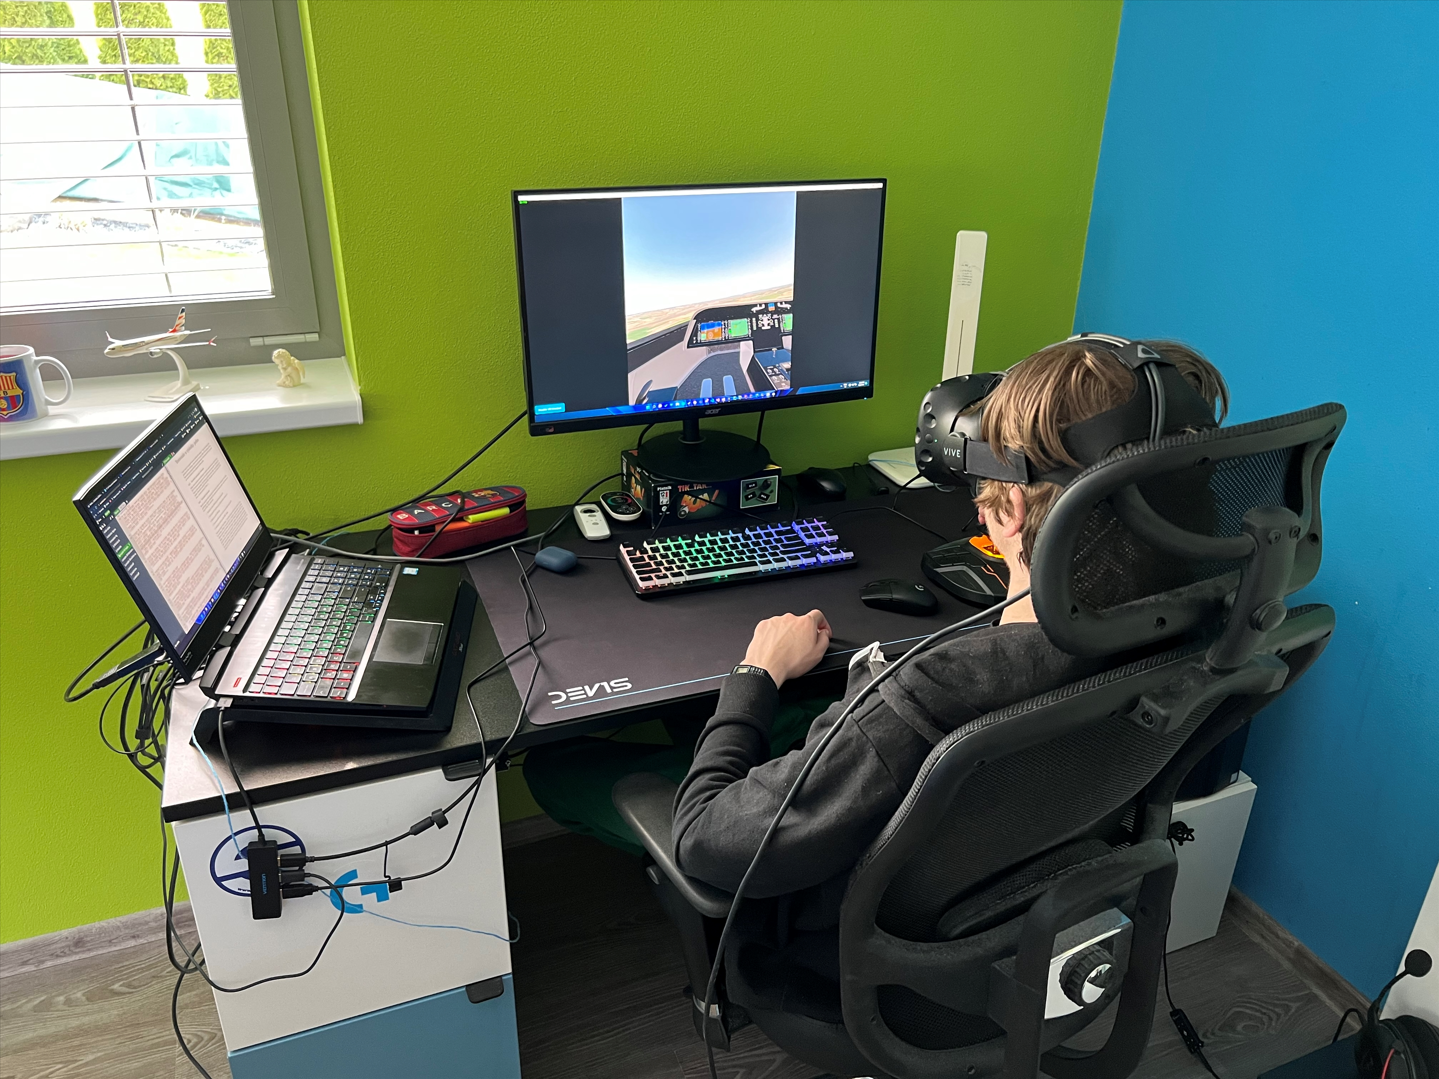
\includegraphics[scale=0.27]{obrazky-figures/uzivatel1.png}
\caption{Uživateľské testovanie letúna v~leteckom simulátore.}{\label{uzivatel1}}
\end{figure}

\begin{figure}[ht]
\centering
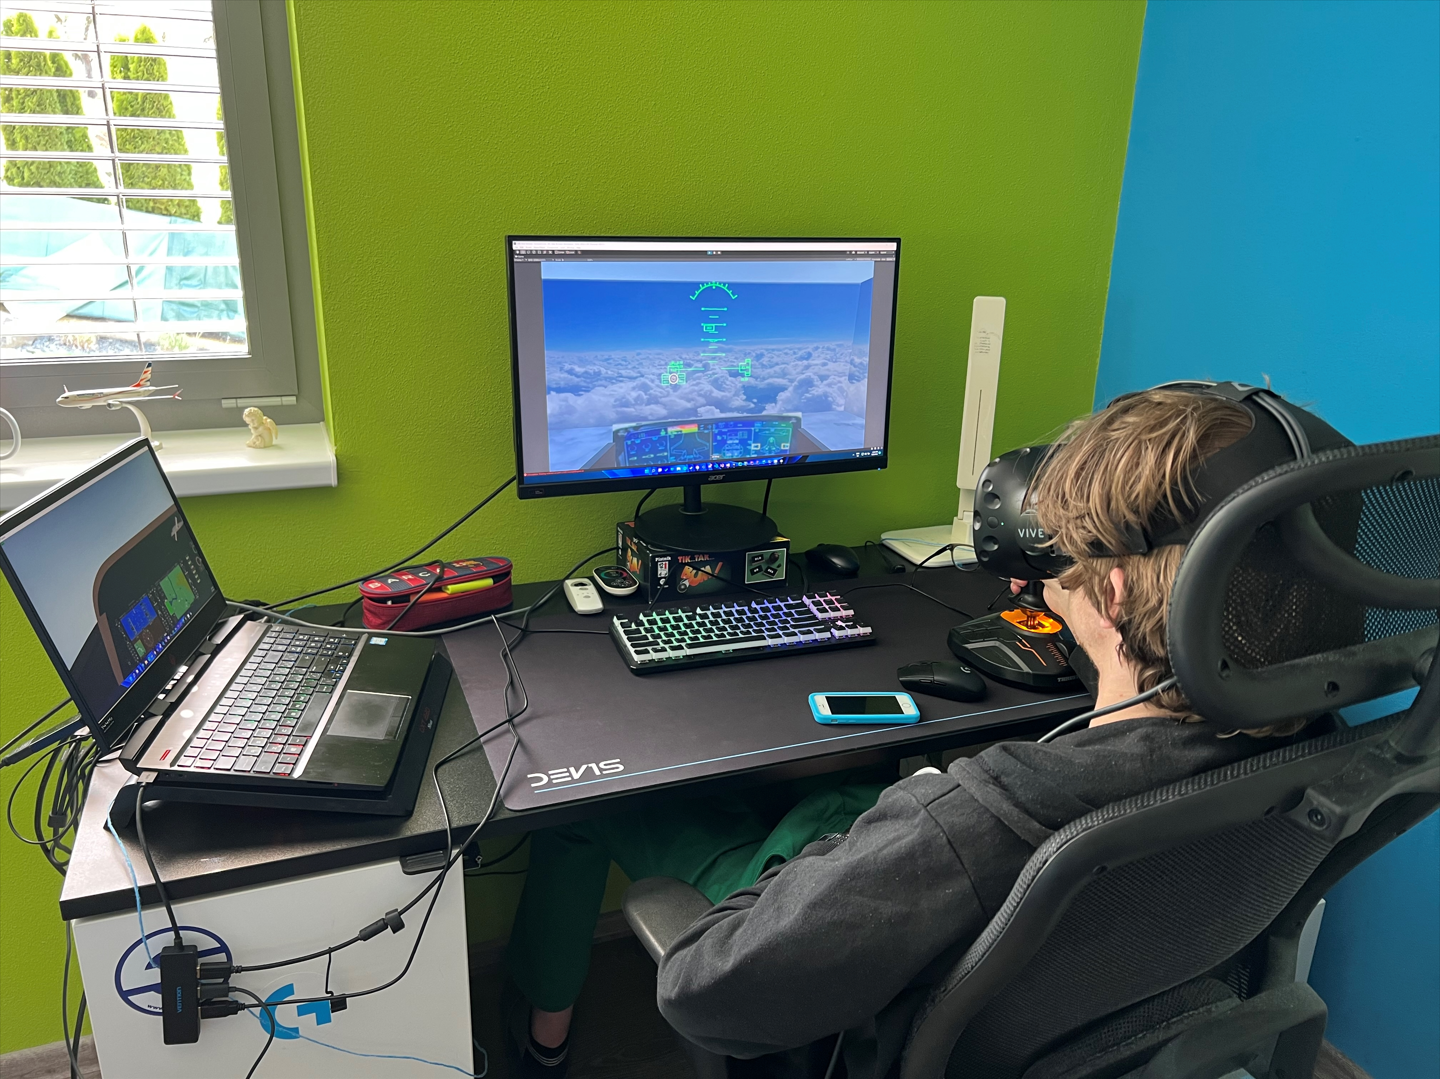
\includegraphics[scale=0.27]{obrazky-figures/uzivatel2.png}
\caption{Uživateľské testovanie HUD.}{\label{uzivatel2}}
\end{figure}

\newpage
\begin{figure}[ht]
\centering
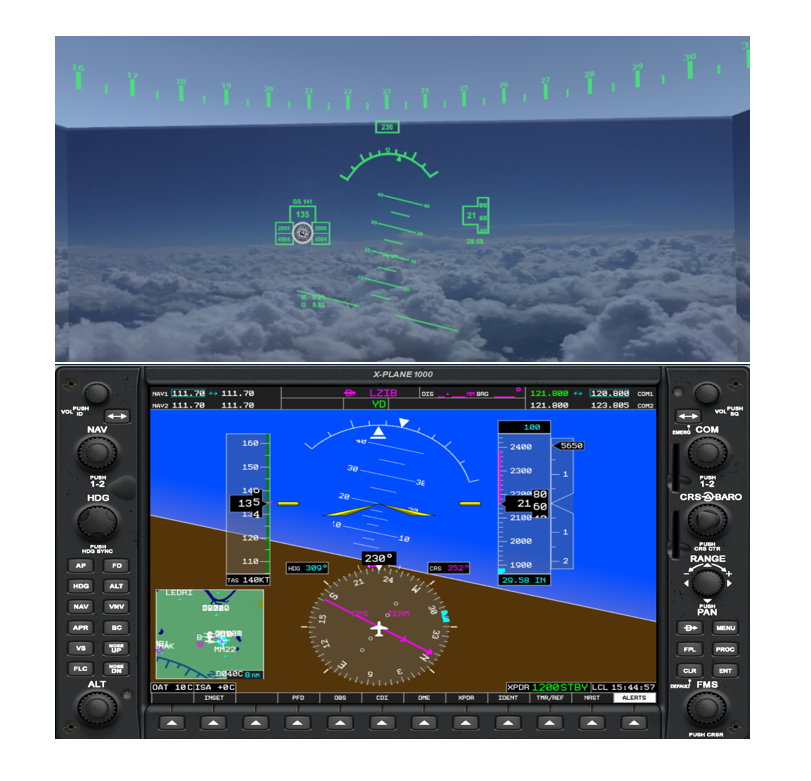
\includegraphics[scale=0.69]{obrazky-figures/porovnanie.png}
\caption{Testovanie HUD na základe porovnania hodnôt so simulátorom X-Plane 11.}{\label{porovnanie}}
\end{figure}

\subsection{Výsledky práce}
Výsledky práce boli zhotovené na základe získaných odpovedí uživateľov z~dotazníka. Hlavným zameraním dotazníka bolo zistiť, aká bola čítateľnosť jednotlivých častí HUD, ako sa im páčila celková štruktúra HUD, či HUD obsahoval všetky časti, ktoré potrebovali počas letu, čo sa im na displeji najviac páčilo alebo naopak nepáčilo a čo by prípadne zmenili alebo doplnili v~priehľadovom displeji. Odpovede respondentov sú znázornené na výsledných grafoch, ktoré sú zobrazené na obrázkoch \ref{dotaznik1.1}, \ref{dotaznik2.1} a \ref{dotaznik3.1}.

\begin{figure}[ht]
\centering
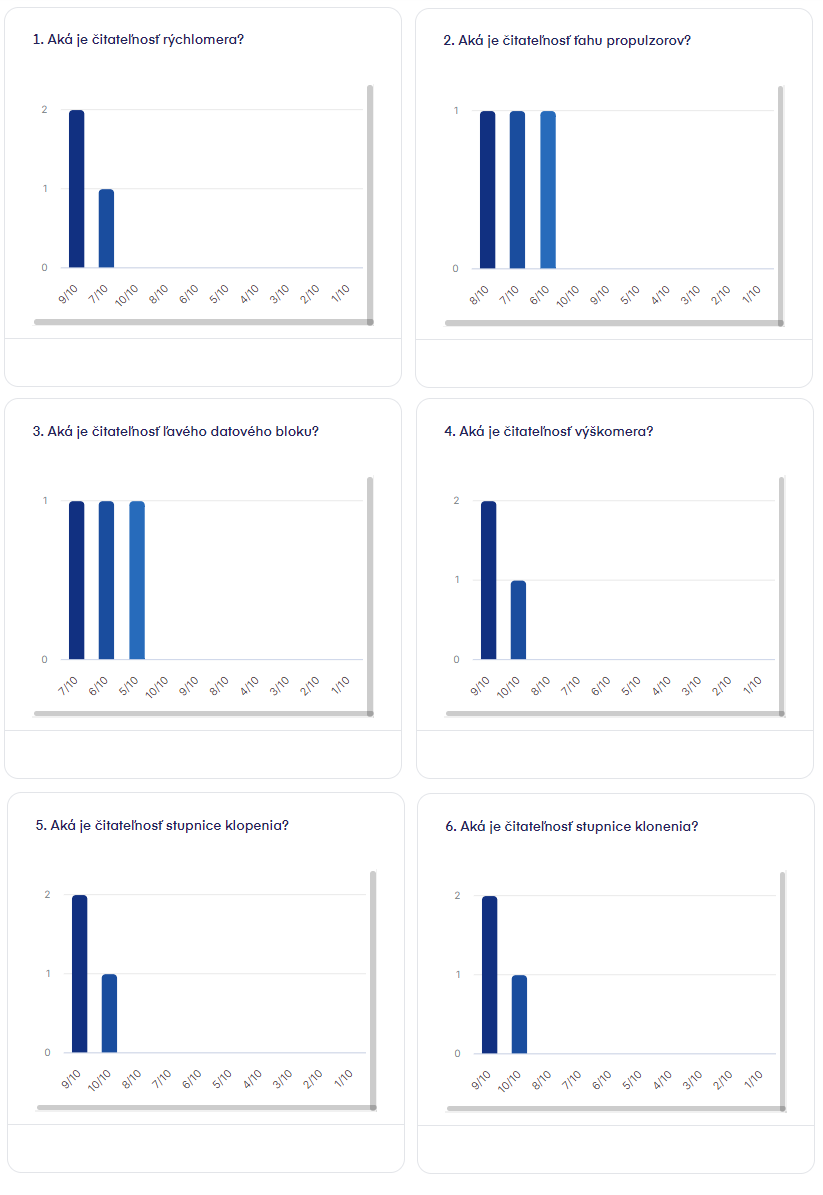
\includegraphics[scale=0.65]{obrazky-figures/dotaznik1.1n.png}
\caption{Výsledky uživateľského testovania, otázky 1-6.}{\label{dotaznik1.1}}
\end{figure}

\begin{figure}[ht]
\centering
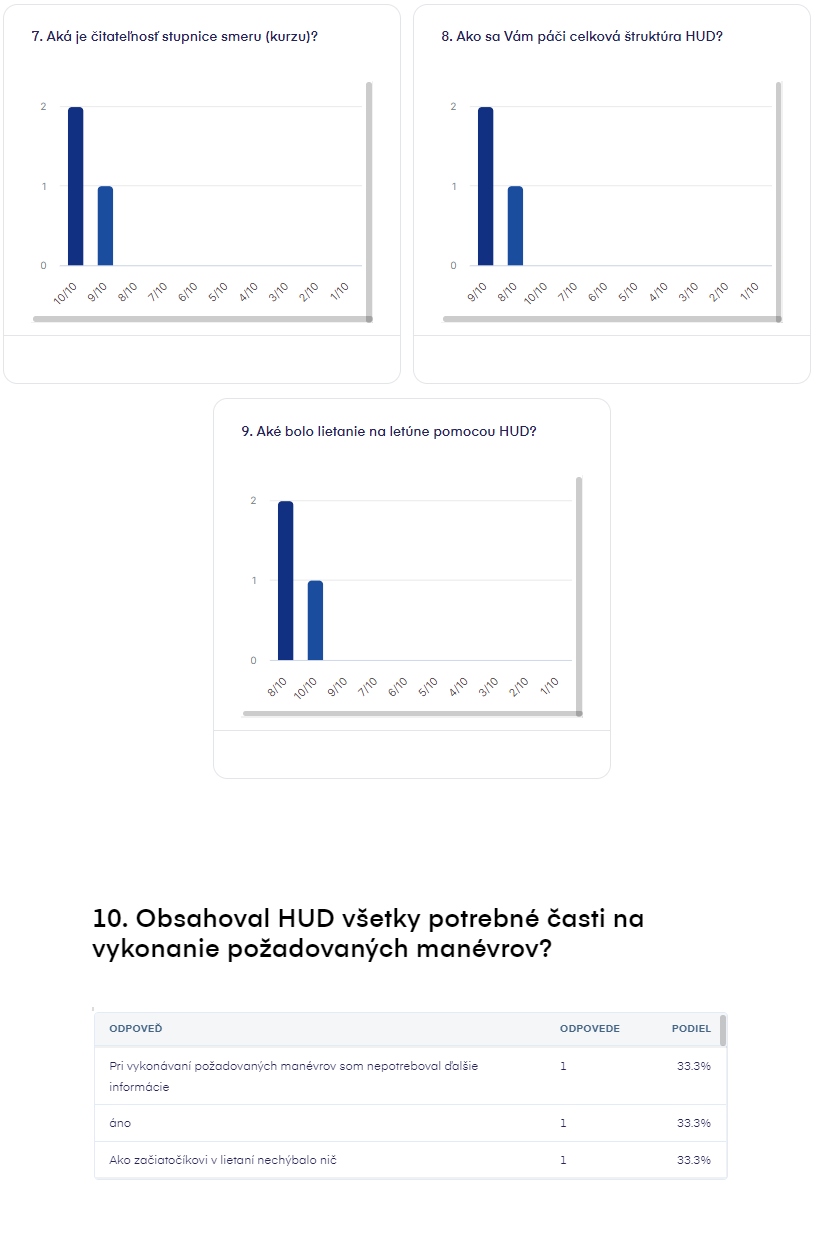
\includegraphics[scale=0.65]{obrazky-figures/dotaznik1.2n.png}
\caption{Výsledky uživateľského testovania, otázky 7-10.}{\label{dotaznik2.1}}
\end{figure}

\begin{figure}[ht]
\centering
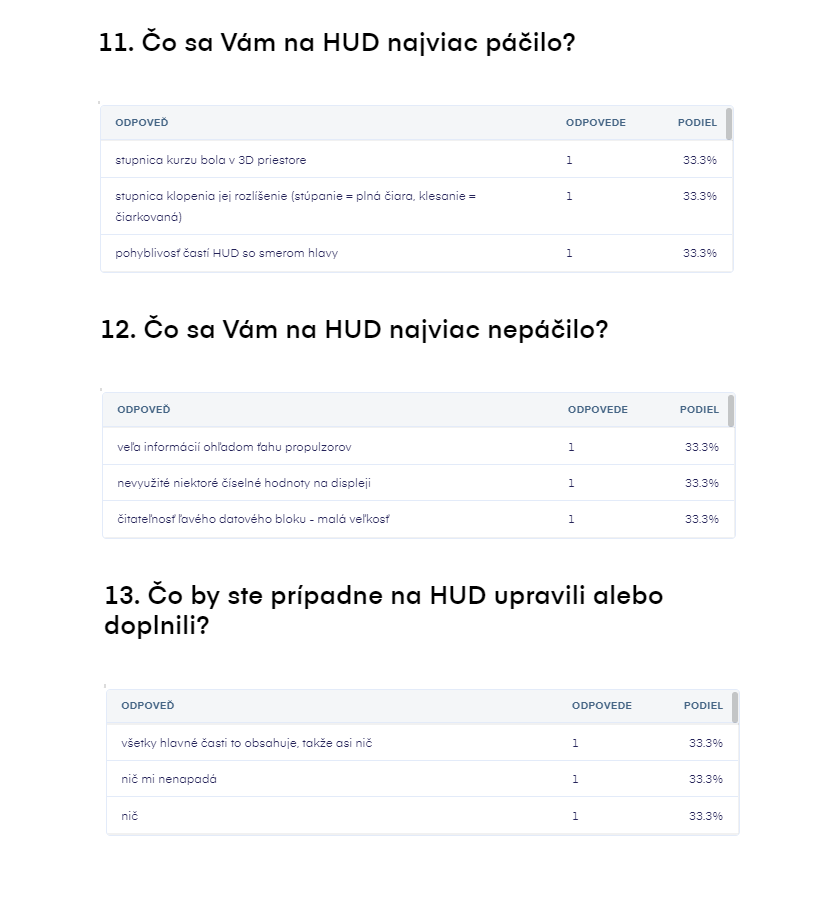
\includegraphics[scale=0.65]{obrazky-figures/dotaznik2.1n.png}
\caption{Výsledky uživateľského testovania, otázky 11-13.}{\label{dotaznik3.1}}
\end{figure}

Pri čítateľnosti sa zistilo, že najlepšie je na tom stupnica smeru, ktorá mala najvýššie hodnotenie zo všetkých častí. Následne sa zistilo, že uživateľom pri vykonávaní manévrom nechýbali žiadne ďalšie informácie a že by na displeji nič nemenili. Najviac sa uživateľom páčila pohyblivosť častí s~hlavou uživateľa, zaoblenie stupnice kurzu do 3D priestoru a~dizajn stupnice klopenia. Z~jednotlivých odpovedí sa dospelo k~záveru, že pomocou HUD bol užívateľ schopný riadiť letún bez problémov.

\chapter{Záver}
%Zaver
Hlavným cieľom tejto bakalárskej práce bolo navrhnúť a implementovať vizualizáciu letových dát pre priehľadový displej v~prostredí leteckého simulátora, ktorý obsahuje technológie podporujúce virtuálnu realitu. Pre vytvorenie návrhu bolo potrebné získať požadované vedomosti z~oblasti súčasných trendov vizualizácie letových dát a naštudovať historický vývoj vizualizácie letových veličín v~pilotnej kabíne. Najväčší dôraz pri tvorbe návrhu bol vkladaný na výber častí obsahujúcich užitočné informácie, ktoré pilot počas letu využíva. Taktiež bolo dôležité navrhnúť správne umiestnenie jednotlivých častí zobrazených na displeji. Po vytvorení návrhu bolo nevyhnutné dať jednotlivým častiam HUD funkcionalitu, ktorá bola implementovaná v~aplikácií Unity. Na naprogramovanie logiky HUD bol použitý programovací jazyk C\#. 

Výsledky testovania a overenie funkčnosti priehľadového displeja bolo vykonané na základe testovania pomocou virtuálnej reality HTC Vive v~leteckom simulátore X-Plane 11. Uživatelia najskôr testovali viacero manévrov v~leteckom simulátore na letúne AG-4 za~pomoci panela prístrojov. Následne vykonali rovnaké manévre v~Unity za pomoci priehľadového displeja. Po~testovaní bol pre uživateľov pripravený dotázník s~otázkami zameranými na čitateľnosť jednotlivých častí priehľadového displeja, štruktúru HUD či dizajn HUD. Na~základe testovania a dotazníka od rôznych užívateľov sa dospelo k~záveru, že uživateľ bol schopný vykonať manévre bez problémov. 

\section{Vývoj v~budúcnosti}
V~budúcnosti by sa na tejto bakalárskej práci dalo pracovať s~vylepšením častí HUD. V~budúcom vývoji by sa dal displej vylepšiť o~možnosť zobrazovania kontrolných údajov ako je kontrolný zoznam. Z~hľadiska zvyšovania prevádzkovej bezpečnosti by sa na displeji mohli pridať bezpečnostné informácie ako sú napríklad chybové hlášky. Zaujímavým doplnkom by taktiež bola možnosť ovládania pomocou gést alebo hlasu, kde by uživateľ mal možnosť meniť rôzne vizualizácie.

  \fi
  
  % Kompilace po částech (viz výše, nutno odkomentovat)
  % Compilation piecewise (see above, it is necessary to uncomment it)
  %\subfile{projekt-01-uvod-introduction}
  % ...
  %\subfile{chapters/projekt-05-conclusion}


  % Pouzita literatura / Bibliography
  % ----------------------------------------------
\ifslovak
  \makeatletter
  \def\@openbib@code{\addcontentsline{toc}{chapter}{Literatúra}}
  \makeatother
  \bibliographystyle{bib-styles/Pysny/skplain}
\else
  \ifczech
    \makeatletter
    \def\@openbib@code{\addcontentsline{toc}{chapter}{Literatura}}
    \makeatother
    \bibliographystyle{bib-styles/Pysny/czplain}
  \else 
    \makeatletter
    \def\@openbib@code{\addcontentsline{toc}{chapter}{Bibliography}}
    \makeatother
    \bibliographystyle{bib-styles/Pysny/enplain}
  %  \bibliographystyle{alpha}
  \fi
\fi
  \begin{flushleft}
  \bibliography{projekt-20-literatura-bibliography}
  \end{flushleft}

  % vynechani stranky v oboustrannem rezimu
  % Skip the page in the two-sided mode
  \iftwoside
    \cleardoublepage
  \fi

  % Prilohy / Appendices
  % ---------------------------------------------
  \appendix
\ifczech
  \renewcommand{\appendixpagename}{Přílohy}
  \renewcommand{\appendixtocname}{Přílohy}
  \renewcommand{\appendixname}{Příloha}
\fi
\ifslovak
  \renewcommand{\appendixpagename}{Prílohy}
  \renewcommand{\appendixtocname}{Prílohy}
  \renewcommand{\appendixname}{Príloha}
\fi
  \appendixpage

% vynechani stranky v oboustrannem rezimu
% Skip the page in the two-sided mode
%\iftwoside
%  \cleardoublepage
%\fi
  
\ifslovak
  \section*{Zoznam príloh}
  \addcontentsline{toc}{section}{Zoznam príloh}
\else
  \ifczech
%    \section*{Seznam příloh}
%    \addcontentsline{toc}{section}{Seznam příloh}
  \else
%    \section*{List of Appendices}
%    \addcontentsline{toc}{section}{List of Appendices}
  \fi
\fi
  \startcontents[chapters]
  \setlength{\parskip}{0pt} 
   %seznam příloh / list of appendices
   \printcontents[chapters]{l}{0}{\setcounter{tocdepth}{2}}
  
  \ifODSAZ
    \setlength{\parskip}{0.5\bigskipamount}
  \else
    \setlength{\parskip}{0pt}
  \fi
  
  % vynechani stranky v oboustrannem rezimu
  \iftwoside
    \cleardoublepage
  \fi
  
  % Přílohy / Appendices
  \ifenglish
    \input{projekt-30-prilohy-appendices-en}
  \else
    %Prílohy

\chapter{Plagát}
\begin{figure}[ht]
\centering
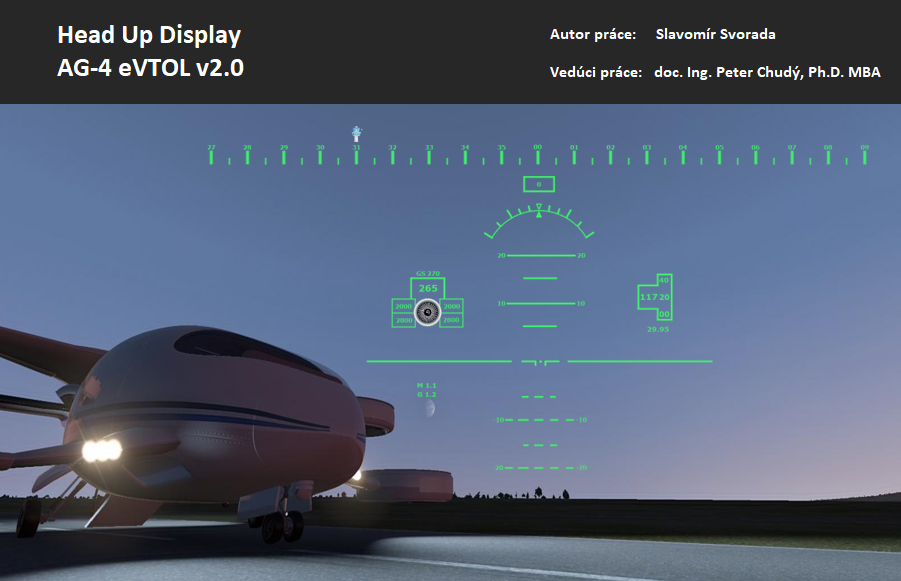
\includegraphics[scale=0.6]{obrazky-figures/plagatFinal.png}
\caption{Plagát prezentujúci priehľadový displej.}{\label{plagat}}
\end{figure}

\chapter{Dotazník k testovaniu}

\noindent

\begin{enumerate}
\item{Aký je Váš vek? \newline
\_\_\_\_\_\_\_\_\_\_\_\_\_\_\_\_\_\_\_\_\_\_\_\_\_\_\_\_\_\_\_\_\_\_\_\_\_\_\_\_\_\_\_\_\_}

\item{Koľko hodín máte nalietaných na leteckom simulátore? \newline
\_\_\_\_\_\_\_\_\_\_\_\_\_\_\_\_\_\_\_\_\_\_\_\_\_\_\_\_\_\_\_\_\_\_\_\_\_\_\_\_\_\_\_\_\_}

\end{enumerate}

\newcolumntype{P}{>{\centering\arraybackslash}p{0.6cm}}
\newcolumntype{L}{>{\raggedright\arraybackslash}m{0.2\textwidth}}
\newcolumntype{R}{>{\raggedleft\arraybackslash}m{0.2\textwidth}}

\newcommand{\printtblhdr}{%
  \hfill
  \begingroup
  \setlength\tabcolsep{0pt}%
  \begin{tabularx}{0.41\textwidth}{ @{} l *{3}X r @{} }
    \multicolumn{2}{l}{\bfseries\shortstack[l]{Zlá}}
    &&
    \multicolumn{2}{l}{\bfseries\shortstack[r]{Výborná}}
    \\
  \end{tabularx}
  \endgroup
}

\newcommand{\usetbl}{%
  \begin{tabular}{ c c c c c c c c c c}
    \hline
    1 & 2 & 3 & 4 & 5 & 6 & 7 & 8 & 9 & 10\\
    \hline
  \end{tabular}
}

\newcommand\prop[1]{%
  \item
  \parbox[t]{0.47\textwidth}{#1}%
  \qquad
  \parbox[t]{0.53\textwidth}{\usetbl}%
}

\printtblhdr

\begin{enumerate}
\setcounter{enumi}{2}
\prop{Aká je čitateľnosť rýchlomera?}

\prop{Aká je čitateľnosť ťahu propulzorov?}

\prop{Aká je čitateľnosť ľavého datového bloku?}

\prop{Aká je čitateľnosť výškomera?}

\prop{Aká je čitateľnosť stupnice klopenia?}

\prop{Aká je čitateľnosť stupnice klonenia?}

\prop{Aká je čitateľnosť stupnice smeru (kurzu)?}


\end{enumerate}
%-----------------------------------------------------------------

\newcolumntype{P}{>{\centering\arraybackslash}p{0.6cm}}
\newcolumntype{L}{>{\raggedright\arraybackslash}m{0.2\textwidth}}
\newcolumntype{R}{>{\raggedleft\arraybackslash}m{0.2\textwidth}}

\newcommand{\printtblhdrr}{%
  \hfill
  \begingroup
  \setlength\tabcolsep{0pt}%
  \begin{tabularx}{0.41\textwidth}{ @{} l *{3}X r @{} }
    \multicolumn{2}{l}{\bfseries\shortstack[l]{Nepáči}}
    &&
    \multicolumn{2}{l}{\bfseries\shortstack[r]{Páči}}
    \\
  \end{tabularx}
  \endgroup
}

\newcommand{\usetbll}{%
  \begin{tabular}{ c c c c c c c c c c}
    \hline
    1 & 2 & 3 & 4 & 5 & 6 & 7 & 8 & 9 & 10\\
    \hline
  \end{tabular}
}

\newcommand\propp[1]{%
  \item
  \parbox[t]{0.47\textwidth}{#1}%
  \qquad
  \parbox[t]{0.53\textwidth}{\usetbll}%
}

\printtblhdrr

\begin{enumerate}
\setcounter{enumi}{9}
\propp{Ako sa Vám páči celková štruktúra HUD?}

\end{enumerate}

%---------------------------------------------------------
\newcommand{\printtblhdrrr}{%
  \hfill
  \begingroup
  \setlength\tabcolsep{0pt}%
  \begin{tabularx}{0.41\textwidth}{ @{} l *{3}X r @{} }
    \multicolumn{2}{l}{\bfseries\shortstack[l]{Zložité}}
    &&
    \multicolumn{2}{l}{\bfseries\shortstack[r]{Jednoduché}}
    \\
  \end{tabularx}
  \endgroup
}

\newcommand{\usetblll}{%
  \begin{tabular}{ c c c c c c c c c c}
    \hline
    1 & 2 & 3 & 4 & 5 & 6 & 7 & 8 & 9 & 10\\
    \hline
  \end{tabular}
}

\newcommand\proppp[1]{%
  \item
  \parbox[t]{0.47\textwidth}{#1}%
  \qquad
  \parbox[t]{0.53\textwidth}{\usetblll}%
}

\printtblhdrrr

\begin{enumerate}
\setcounter{enumi}{10}
\proppp{Aké bolo lietanie na letúne pomocou HUD?}

\end{enumerate}

%--------------------------------------
\begin{enumerate}
\setcounter{enumi}{11}
\item{Obsahoval HUD všetky potrebné časti na vykonanie požadovaných manévrov? \newline
\_\_\_\_\_\_\_\_\_\_\_\_\_\_\_\_\_\_\_\_\_\_\_\_\_\_\_\_\_\_\_\_\_\_\_\_\_\_\_\_\_\_\_\_\_}
\item{Čo sa Vám na HUD najviac páčilo? \newline
\_\_\_\_\_\_\_\_\_\_\_\_\_\_\_\_\_\_\_\_\_\_\_\_\_\_\_\_\_\_\_\_\_\_\_\_\_\_\_\_\_\_\_\_\_}
\item{Čo sa Vám na HUD najviac nepáčilo? \newline
\_\_\_\_\_\_\_\_\_\_\_\_\_\_\_\_\_\_\_\_\_\_\_\_\_\_\_\_\_\_\_\_\_\_\_\_\_\_\_\_\_\_\_\_\_}
\item{Čo by ste prípadne na HUD upravili alebo doplnili? \newline
\_\_\_\_\_\_\_\_\_\_\_\_\_\_\_\_\_\_\_\_\_\_\_\_\_\_\_\_\_\_\_\_\_\_\_\_\_\_\_\_\_\_\_\_\_}
\end{enumerate}

\chapter{Obsah priloženého pamäťového média}
\begin{DESCRIPTION}
  %\item [data/] - dátové sady použité v experimentoch 
  \item [doc/] - zdrojové súbory tohto textu
  \item [src/] - zdrojové súbory implementovaného priehľadového displeja
  \item [poster/] - plagát prezentujúci priehľadový displej
  \item [video/] - video priehľadového displeja
  \item [BP.pdf] - elektronická verzia tohto textu
\end{DESCRIPTION}
  \fi
  
  % Kompilace po částech (viz výše, nutno odkomentovat)
  % Compilation piecewise (see above, it is necessary to uncomment it)
  %\subfile{projekt-30-prilohy-appendices}

\end{document}
